

% !TEX encoding = UTF-8 Unicode




\usepackage{float}

\documentclass[conference,compsoc]{IEEEtran}

\usepackage{graphicx}
\usepackage{epstopdf}
\DeclareGraphicsExtensions{.eps}
\usepackage{url}
\usepackage{multicol}







\ifCLASSOPTIONcompsoc

\usepackage[nocompress]{cite}
\else
% normal IEEE
\usepackage{cite}
\fi

\ifCLASSINFOpdf

\else

\fi



% correct bad hyphenation here
\hyphenation{op-tical net-works semi-conduc-tor}

\usepackage[utf8x]{inputenc} 



\usepackage{float}
\usepackage{listings}

\usepackage{array}
\newcolumntype{L}[1]{>{\raggedright\let\newline\\\arraybackslash\hspace{0pt}}m{#1}}
\newcolumntype{C}[1]{>{\centering\let\newline\\\arraybackslash\hspace{0pt}}m{#1}}
\newcolumntype{R}[1]{>{\raggedleft\let\newline\\\arraybackslash\hspace{0pt}}m{#1}}

\begin{document}
%
% paper title
% Titles are generally capitalized except for words such as a, an, and, as,
  % at, but, by, for, in, nor, of, on, or, the, to and up, which are usually
  % not capitalized unless they are the first or last word of the title.
  % Linebreaks \\ can be used within to get better formatting as desired.
  % Do not put math or special symbols in the title.
  \title{Study of QoS and Traffic Control Mechanisms in IP Networks}

  % author names and affiliations
  % use a multiple column layout for up to three different
  % affiliations
  \author{\IEEEauthorblockN{Filipe Oliveira, João Rua, Miguel Zenha}
    \IEEEauthorblockA{Computer Science Department\\
      Universidade do Minho\\
        Email: a57816@alunos.uminho.pt, a41841@alunos.uminho.pt, a66551@alunos.uminho.pt,}
  }

% make the title area
\maketitle

% As a general rule, do not put math, special symbols or citations
% in the abstract
\begin{abstract}
In traditional networks, all connections and services get the same treatment. However, since network resources are limited, and the overall Internet only offers a "Best-Effort" approach, it is important to differentiate between connection classes, and to be able to treat them accordingly to standardised and well documented parameters. \par 
This exploratory essay focus on developing a comparative study of traffic control mechanisms in IP networks and corresponding parametrisation,
     using the Network Simulator NS-2. In order to do so, a test platform will be presented and several Diffserv parameters will be discussed.
     \end{abstract}

     \IEEEpeerreviewmaketitle

     \section{Network topology to be used}

     The network topology to be used as test platform is illustrated in figure \ref{fig:network}. The network topology includes six clients (from Cli1 to Cli6), two edge routers (E1 and E2), and a core router (C0). The clients' access links have a capacity of 5Mbps and a delay of 5ms, and the core network links have a capacity of 5Mbps and a delay of 10ms.\par 

     \begin{figure}[H]
     \centering
     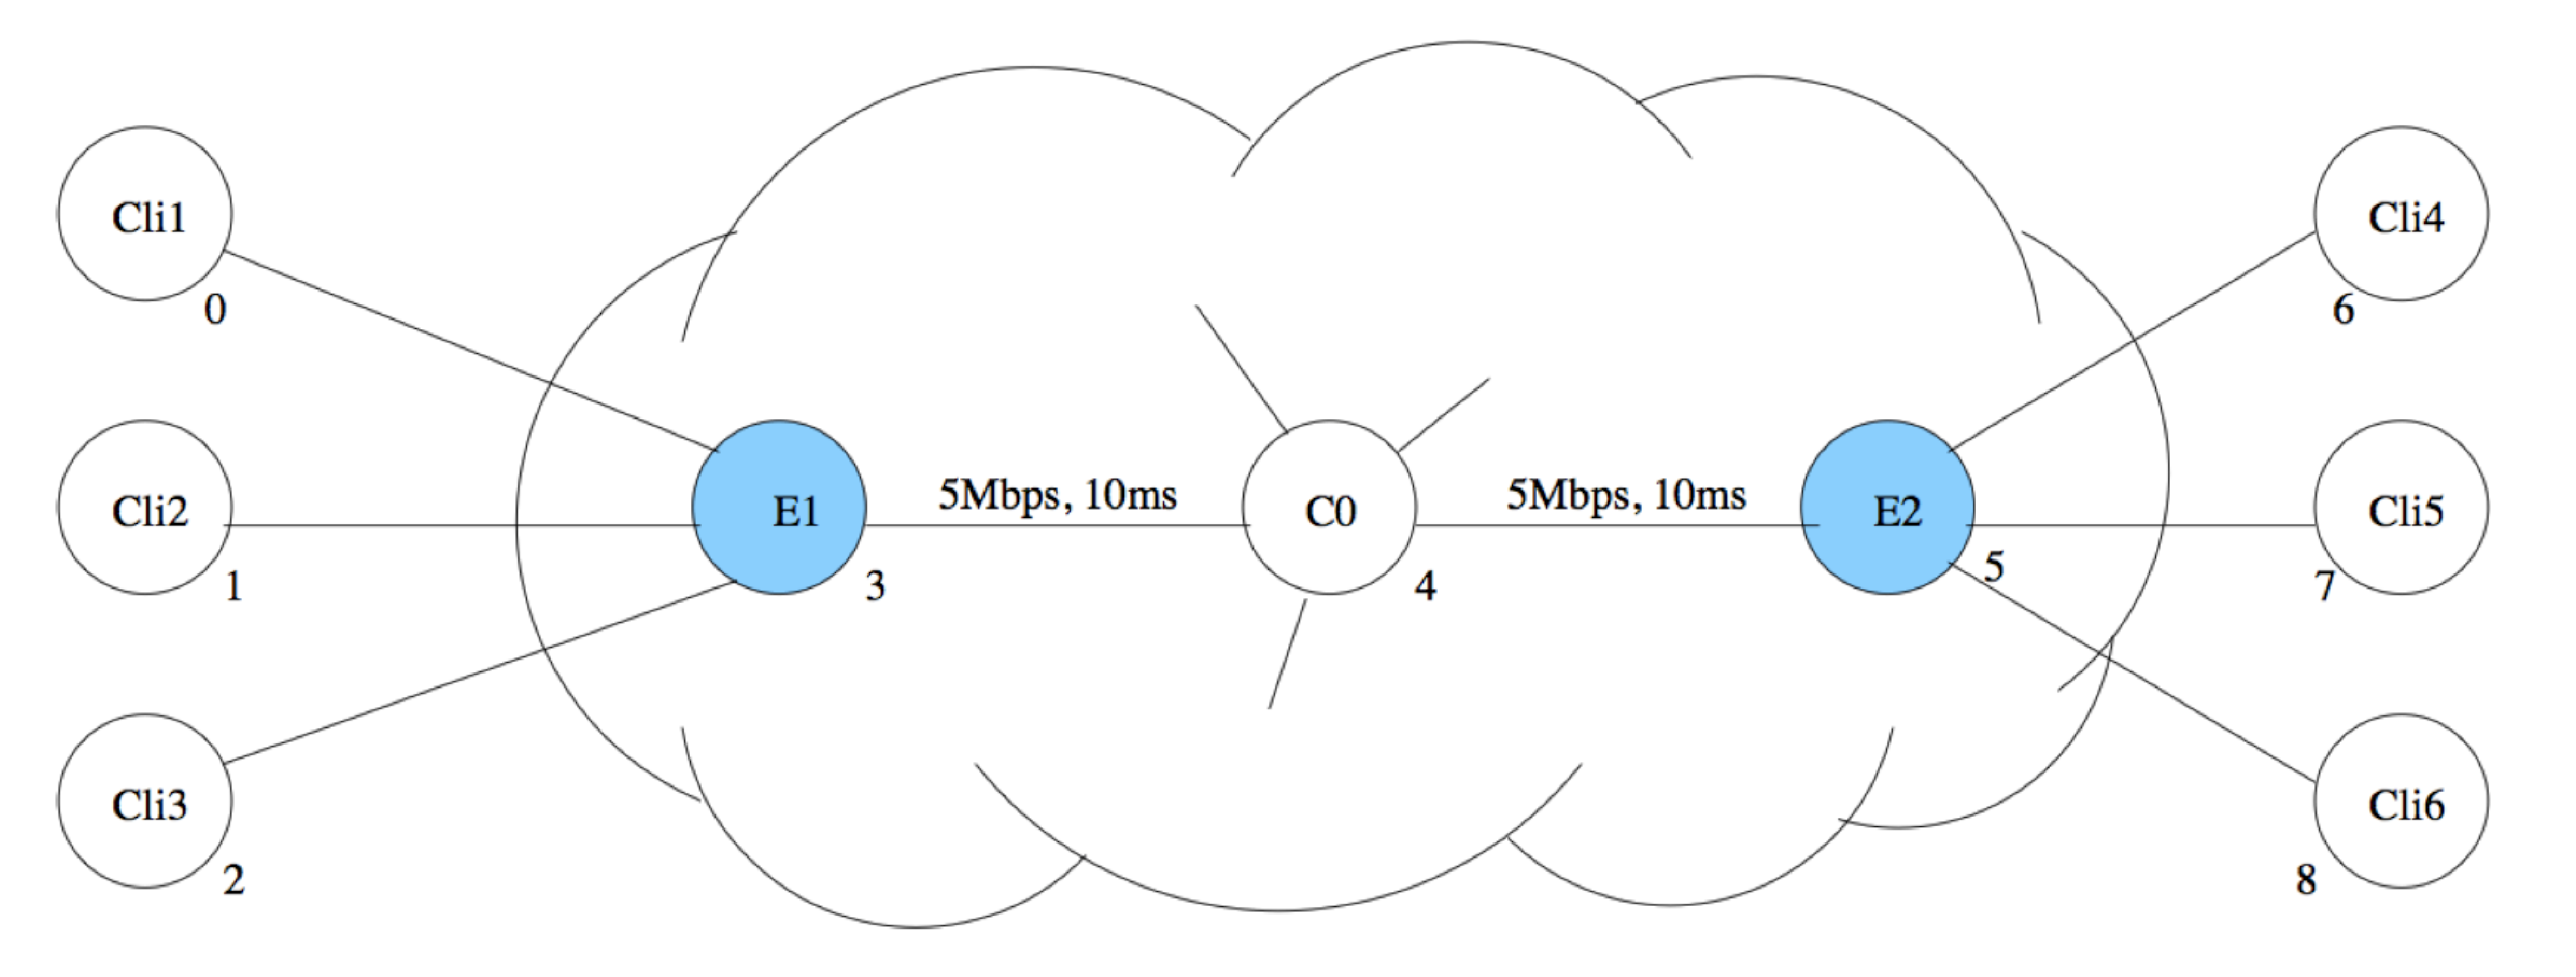
\includegraphics[width=1\columnwidth]{PNG/network.png}
     \caption{ISP network topology}
     \label{fig:network}
     \end{figure}

     The topology is deliberately symmetric to simplify traffic analysis.
     During this exploratory essay several changes will be made regarding the services/applications that every Client holds, however, the topology remains unchanged. \par 
     In most of the cases, it will be enough to analyse flow in one way, however, in the last analyse on chapter \ref{c5}, flows in both ways will be analysed due to the bigger complexity of the simulation.\par 
     As the topology evidences, if all clients use the link capacity simultaneously then congestion will occur in the network backbone, and the service provider will not be able to guarantee proper traffic delivery. To minimise or solve this effect, several traffic control mechanisms will be used in order to promote quality of service (QoS) in the domain.\par 
     Simulations for all scenarios were 15 seconds long. This was a very short simulation time, but enabled us to achieve a confidence interval, producing a stable final state.

     \section{Applications/Services to be used}

     \begin{itemize}
     \item \textbf{CBR over UDP} - generates Constant Bit Rate (CBR) traffic over UDP. This may correspond to
     the transmission of audio or video traffic at a regular/periodic rate.
     \begin{itemize}
     \item Parameters: rate (bits/sec) e packet size (Bytes);
     \end{itemize}
     \item \textbf{FTP} - transfer of large files over TCP;
     \item \textbf{Voice over UDP} - simulates a voice call over UDP; This traffic is characterised by having a constant
     rate, alternating between talk and silence time periods.
     \begin{itemize}
     \item Parameters: rate (bits/sec) and burst size (in seconds).
     \end{itemize}
     \end{itemize}


     \section{Tools and evaluation metrics}
     In order to infer the network quality of service we will take in consideration the following parameters 
     Metrics to use in the simulations:
     \begin{itemize}
     \item \textbf{Loss rate} (total and per flow), in packets/sec.
     \item \textbf{Bandwidth} in use (total and per flow), in bits/sec.
     \end{itemize}

     \section{A - Simulating the "Best-Effort" scenario}
\label{besteffort}
     By default, routers handle packets based on a simple FIFO queueing system, trying to forward them in
     the best possible way according to the available resources (memory and CPU). \par This well-known model is called Best-Effort as there are \textbfno QoS guarantees} on packet delivery (in terms of bounded delays, loss
         and/or bandwidth utilisation). \par 
     For a first approach we considered similar clients with CBR applications,  generating each one a rate of 3Mbps, for a total of six flows (0 $ \rightarrow $ 8, 1 $ \rightarrow $ 7, 2 $ \rightarrow $ 6, 8 $ \rightarrow $0, 7 $ \rightarrow $1,    6 $ \rightarrow $2).\par 

     \subsection{Identification of the links under congestion}

     Producing the graphs illustrating the levels of loss and bandwidth
     utilisation along the time, we can infer that the core network links ( 3 $ \leftrightarrow $ 4, 4 $ \leftrightarrow $ 5 ), since the full bandwidth is being used, as stated in figures \ref{graph:bw_a2} and \ref{graph:loss_a2}.

     \begin{figure}[H]
     \centering
     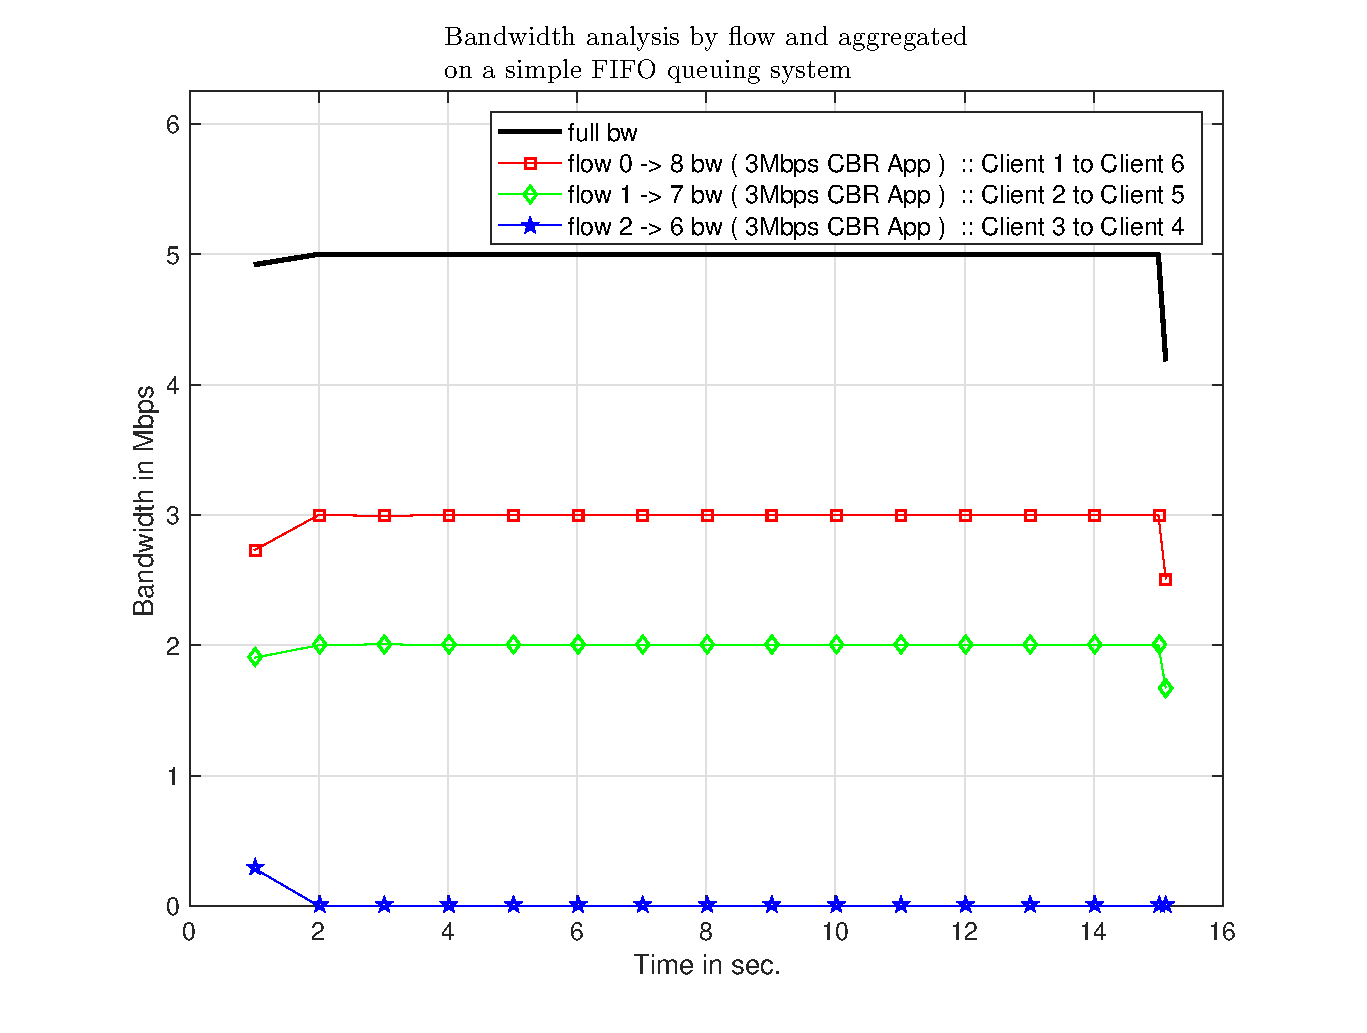
\includegraphics[width=1\columnwidth]{EPS/A/bw_a2.eps}
     \caption{Bandwidth analysis by flow and aggregated on a simple FIFO queueing system, simulation a "best effort" scenario}
     \label{graph:bw_a2}
     \end{figure}


     \begin{figure}[H]
     \centering
     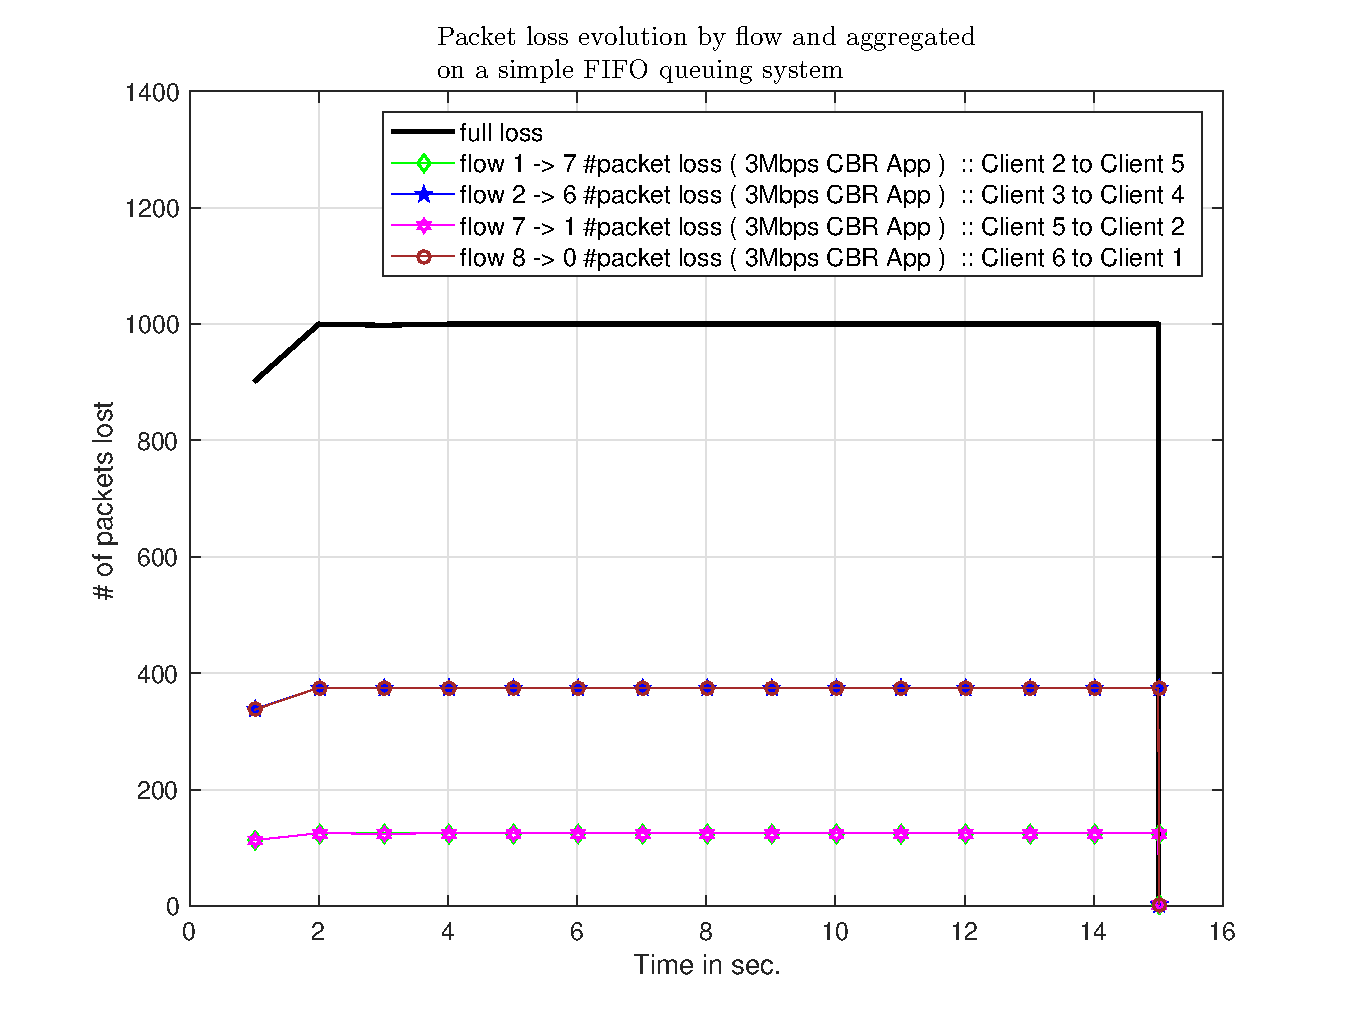
\includegraphics[width=1\columnwidth]{EPS/A/loss_a2.eps}
     \caption{Packet loss evolution by flow and aggregated on a simple FIFO queueing system, simulation a "best effort" scenario}\label{graph:loss_a2}
     \end{figure}

     As stated before, the Internet's "best-effort" scenario produces an undesired non-equitable bandwidth distribution. Denote that this simple simulation only deals with one type of service simulation. The inclusion of other, "more sensible" to network congestion, services like for example VOIP, would result in an unacceptable QoS.\par
     Changing the queues associated with the links under congestion from DropTail to RED would theoretically result into in a better service. The corresponding results are shown in figures \ref{graph:bw_a2_red} and \ref{graph:loss_a2_red}.

     \begin{figure}[H]
     \centering
     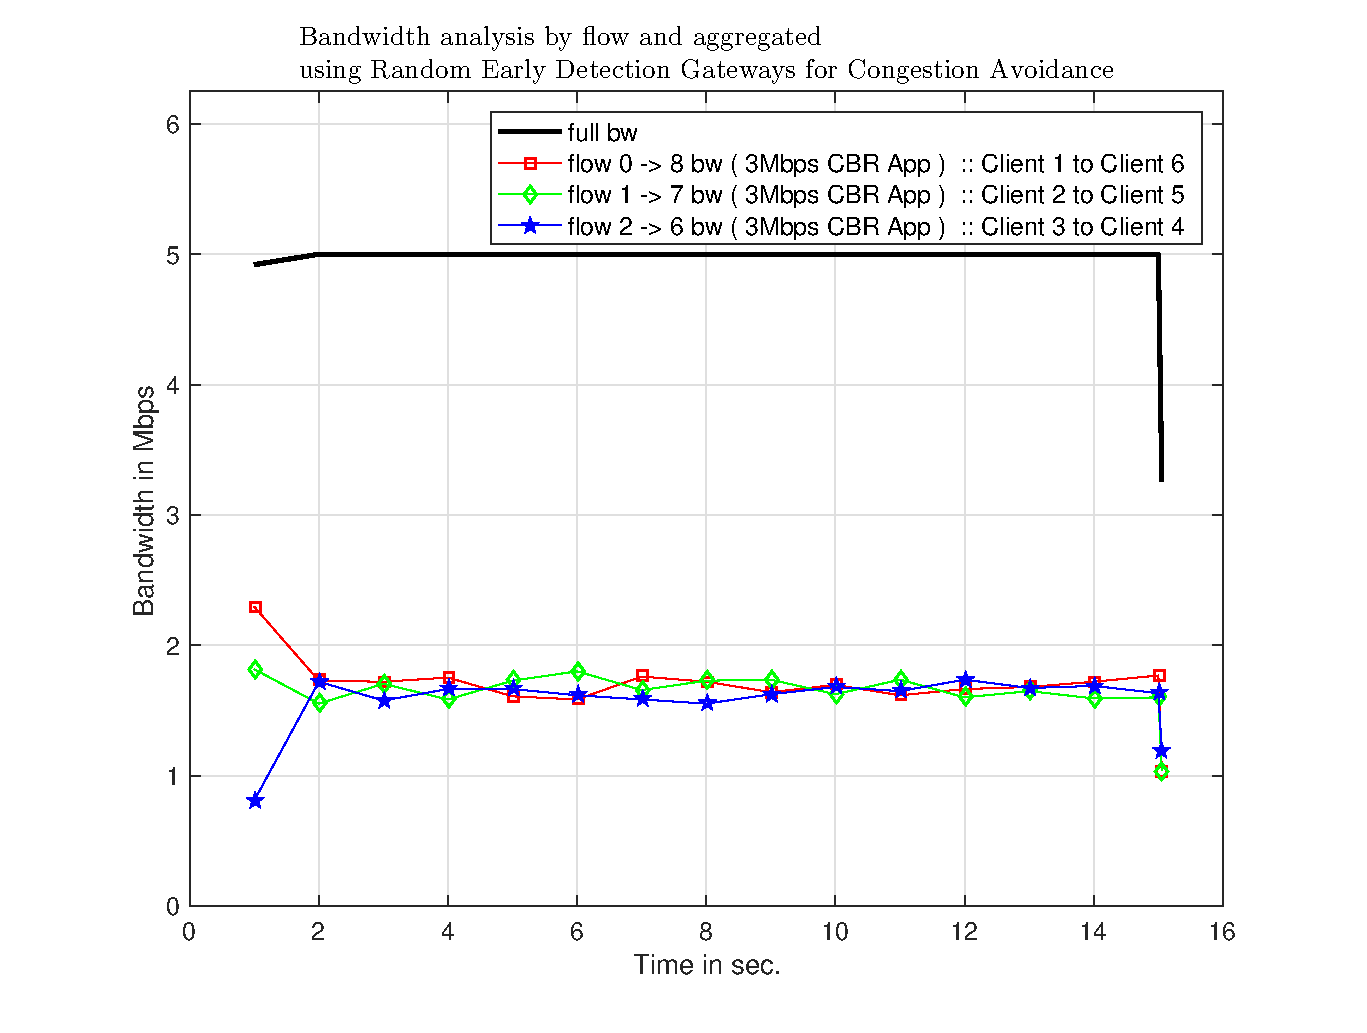
\includegraphics[width=1\columnwidth]{EPS/A/bw_a2_red.eps}
     \caption{Bandwidth analysis by flow and aggregated on a simple FIFO queueing system, simulation a "best effort" scenario, using Random Early Detection Gateways for Congestion Avoidance}
     \label{graph:bw_a2_red}
     \end{figure}


     \begin{figure}[H]
     \centering
     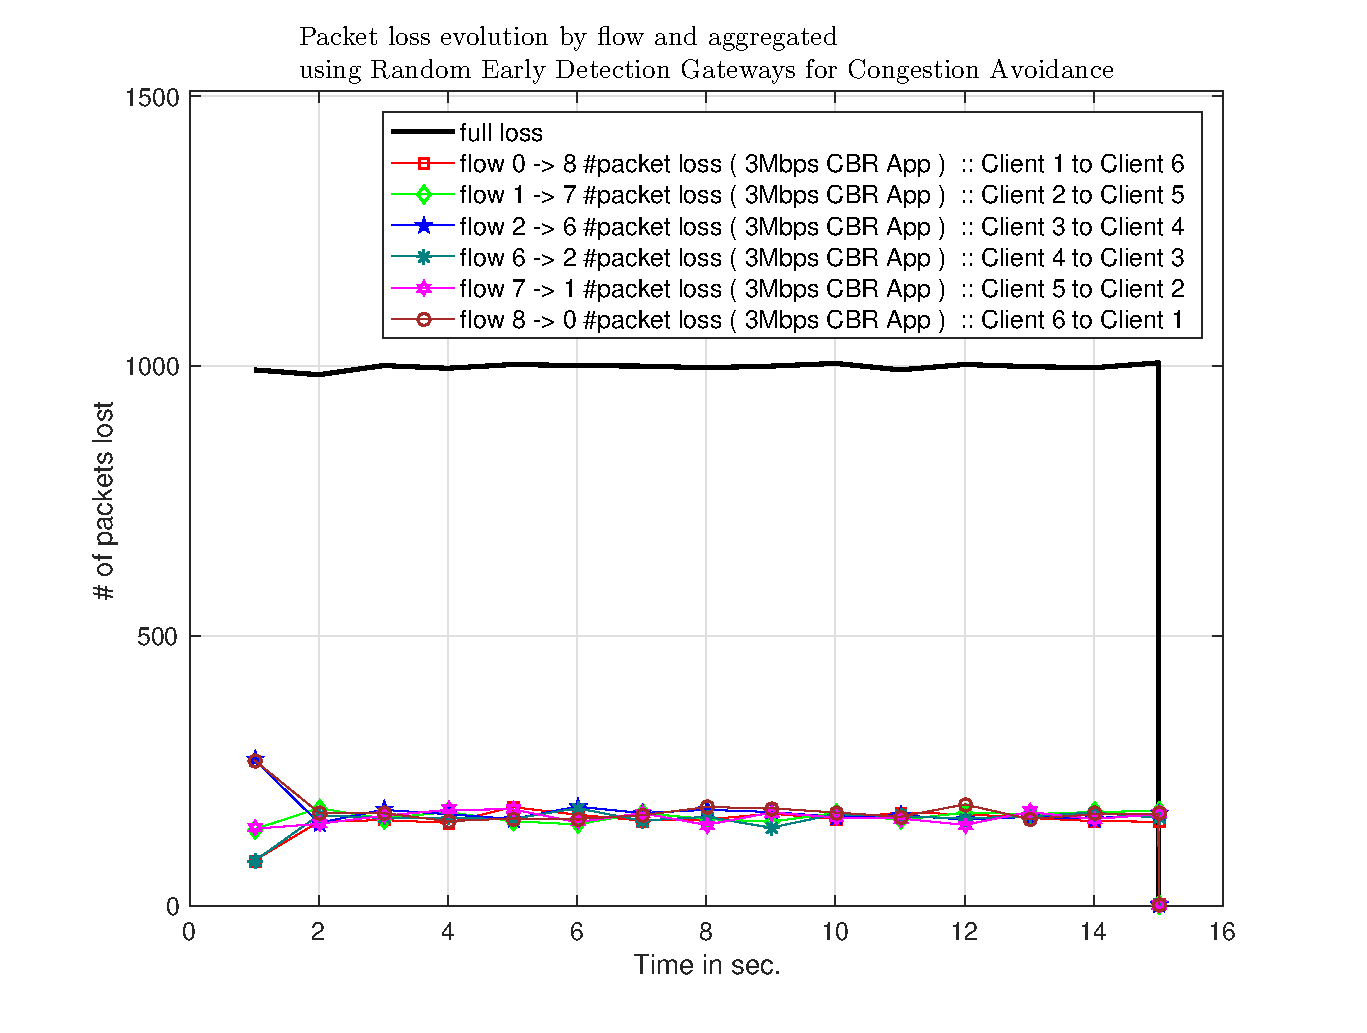
\includegraphics[width=1\columnwidth]{EPS/A/loss_a2_red.eps}
     \caption{Packet loss evolution by flow and aggregated on a simple FIFO queueing system, simulation a "best effort" scenario, using Random Early Detection Gateways for Congestion Avoidance}\label{graph:loss_a2_red}
     \end{figure}

     Notice that this "solution" only improves the equitable bandwidth distribution across flow because they all are produced with the same service/traffic type. If we included for exemplo some TCP over IP service, since it behaves in order to prevent/diminish congestion, it would suffer more from  bandwidth "starvation" than any service using UDP over IP. \par
     In figures   \ref{graph:bw_a3} and \ref{graph:loss_a3}, simulated results are show if one client would generate more CBR traffic than
     the others, on a simple FIFO queuing system, simulating a "best effort" scenario.

     \begin{figure}[H]
     \centering
     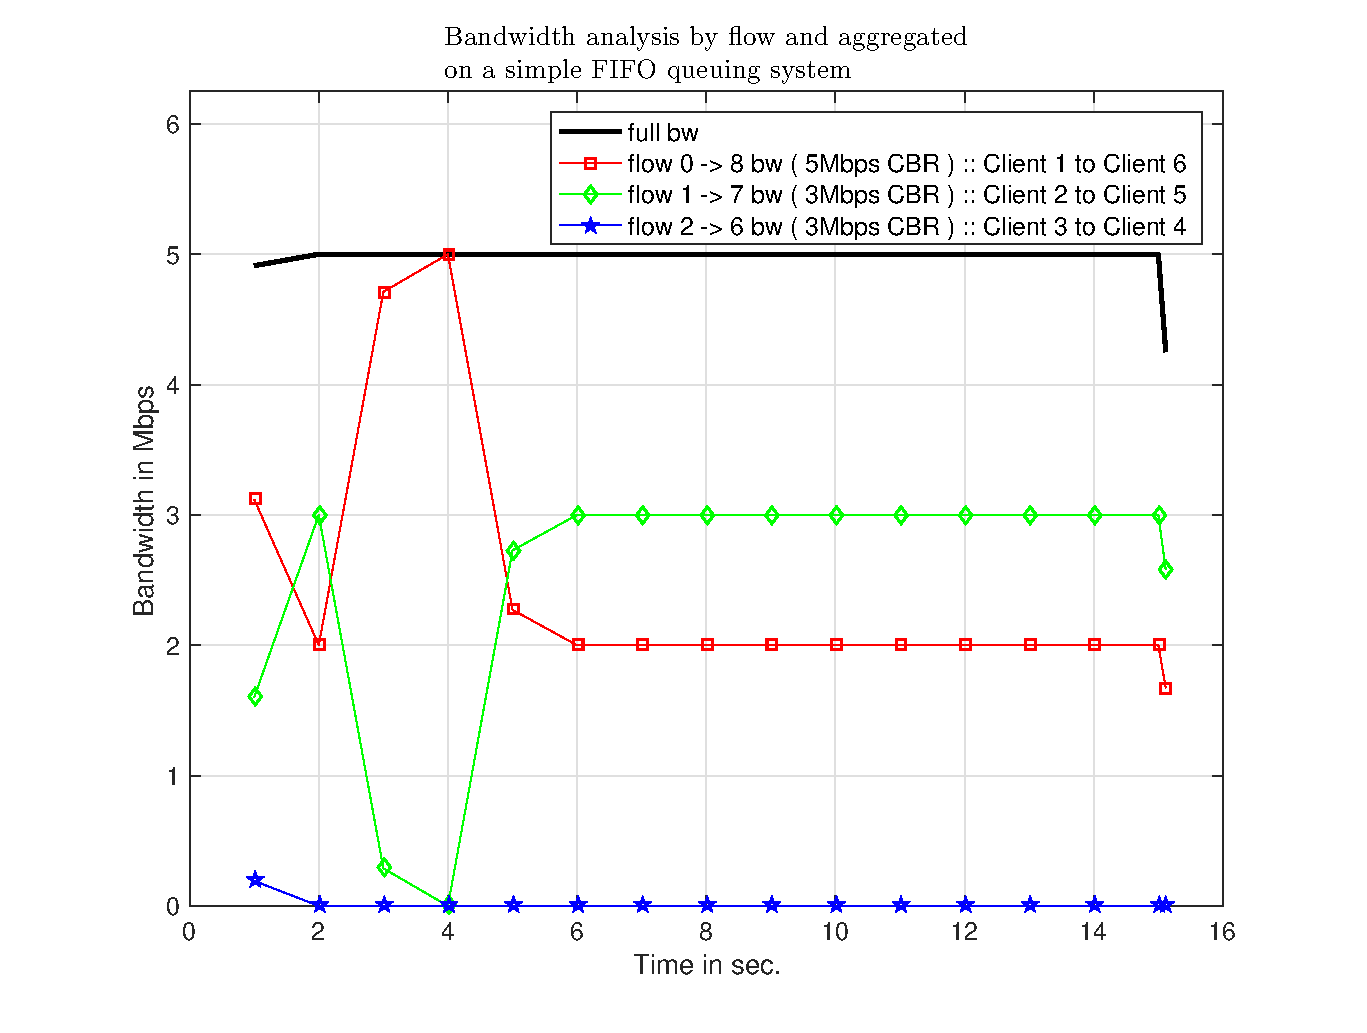
\includegraphics[width=1\columnwidth]{EPS/A/bw_a3.eps}
     \caption{Bandwidth analysis by flow and aggregated on a simple FIFO queueing system, simulation a "best effort" scenario,  in which one client would generate more CBR traffic than the others.}
     \label{graph:bw_a3}
     \end{figure}


     \begin{figure}[H]
     \centering
     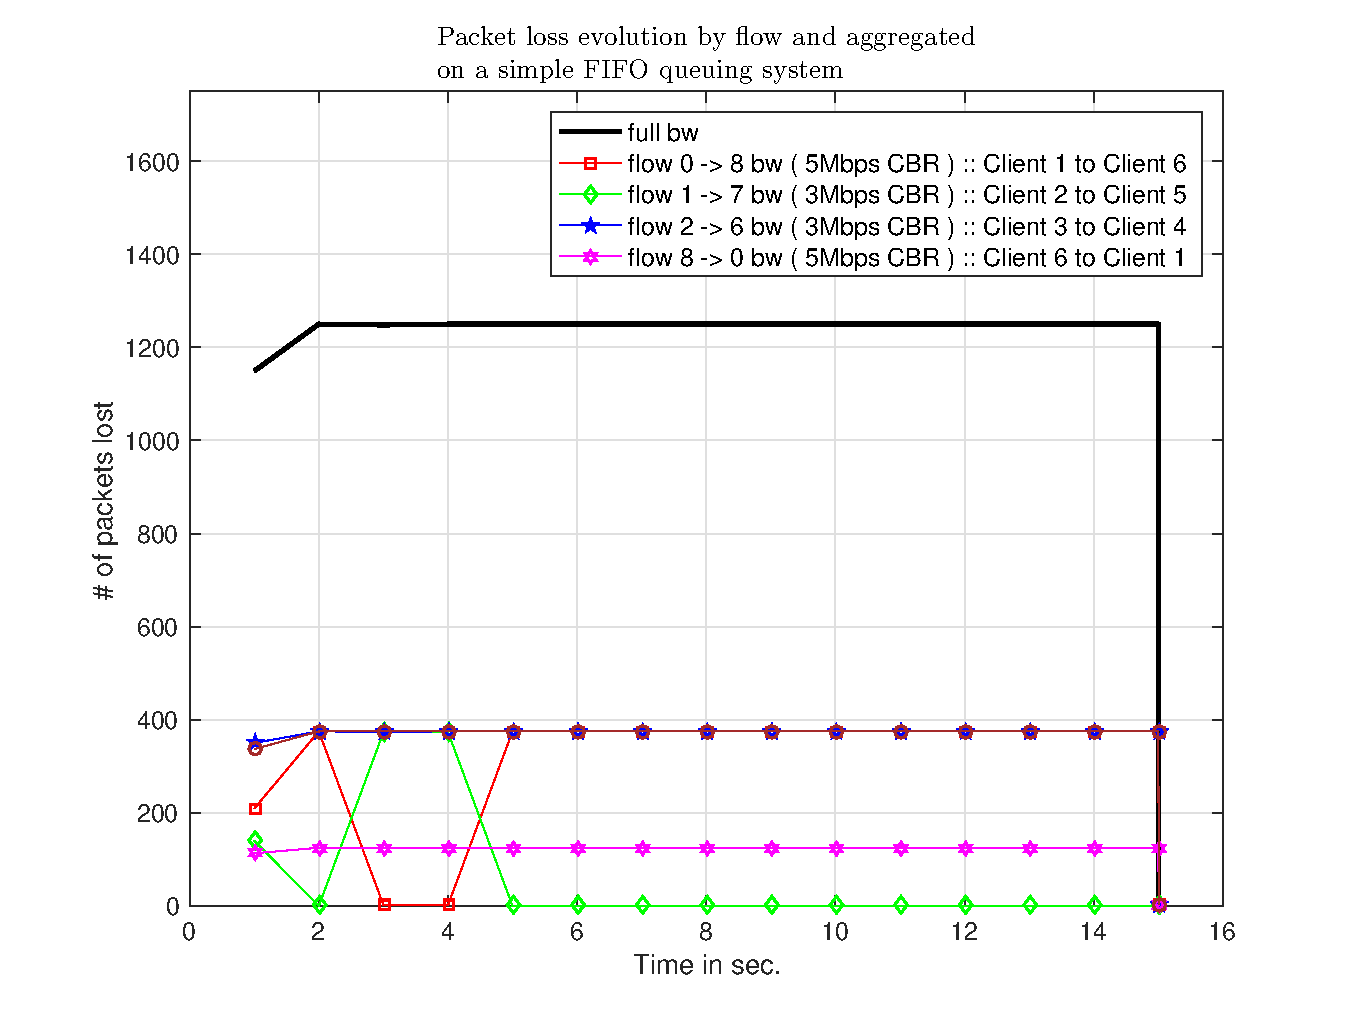
\includegraphics[width=1\columnwidth]{EPS/A/loss_a3.eps}
     \caption{Packet loss evolution by flow and aggregated on a simple FIFO queueing system, simulation a "best effort" scenario,  in which one client would generate more CBR traffic than the others.}\label{graph:loss_a3}
     \end{figure}


     \section{B - Simulating a multi-service network in  the "Best-Effort" scenario}
\label{multiservice}


     In a more realistic scenario, it would be expectable to have both UDP and TCP traffic with other characteristics (FTP, HTTP, etc.).
     Using the procedures already included in the simulation script, several changes were made in order to obtain the
     following scenario:
     \begin{itemize}
     \item a \textbf{CBR application} sending 4Mbps from client 1 to client 6, and other from client 6 to client 1;
     \item  a \textbf{FTP connection} from client 2 to client 5, and other from client 4 to client 2;
     \item  a \textbf{voice connection over UDP} from client 3 to client 4, and vice-versa. Since VOIP Bandwidth consumption naturally depends on the codec used, we selected G.711 - 64 Kbps Bitrate and 87.2 Kbps Nominal Ethernet Bandwidth, and simulated a maximum of 30 calls at any given simulation time. The presented graphic results for VOIP are an aggregation of all the 30 calls. 
     \end{itemize}
     The corresponding results are shown in figures \ref{graph:bw_b1} and \ref{graph:loss_b11}.

     \begin{figure}[H]
     \centering
     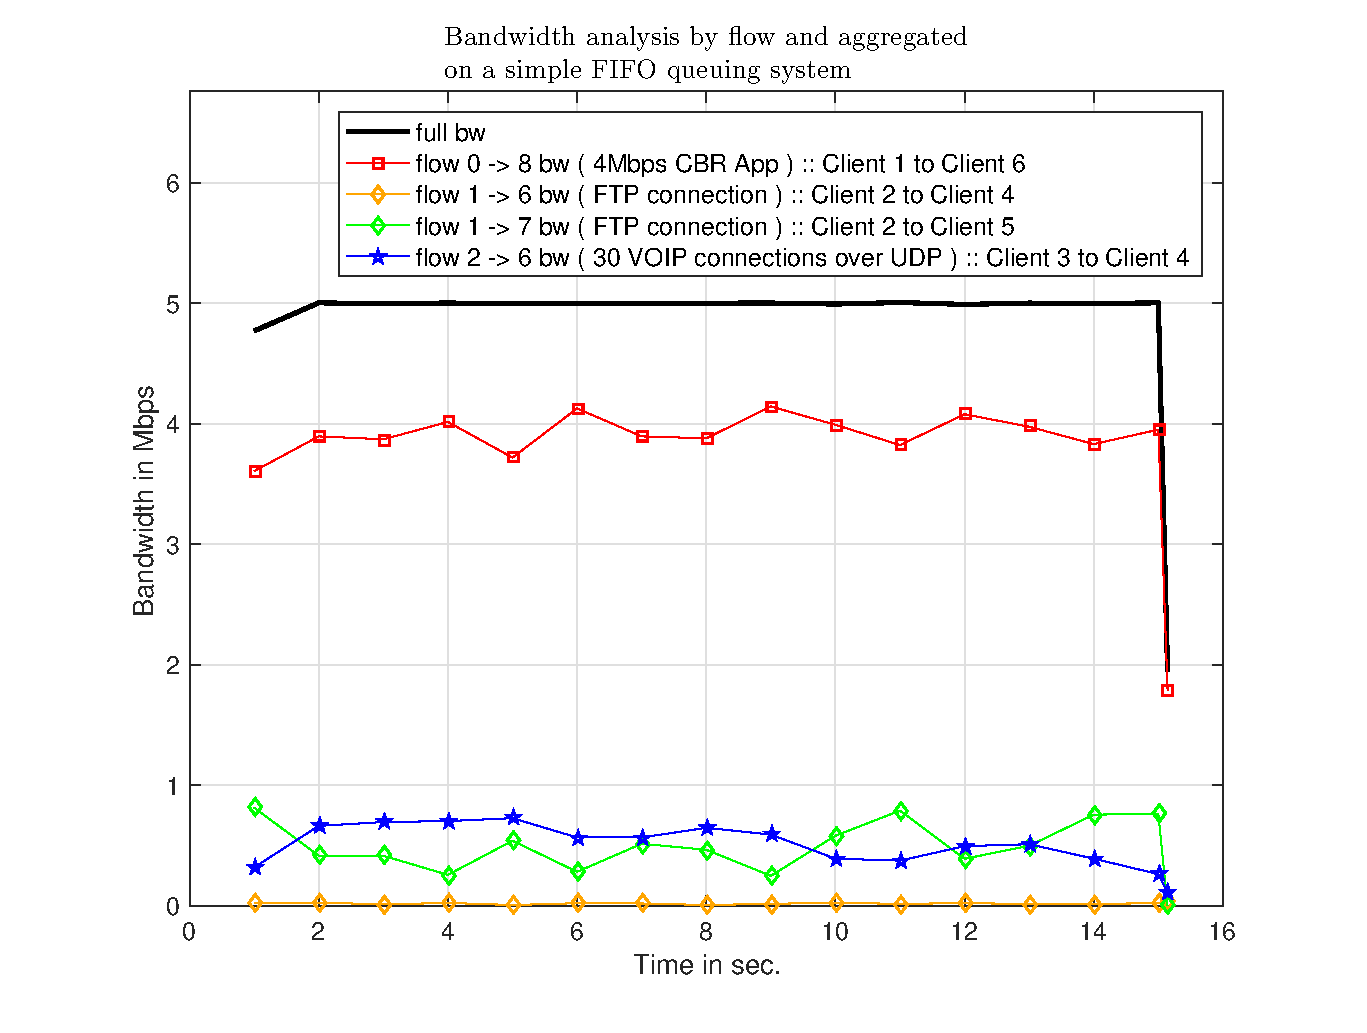
\includegraphics[width=1\columnwidth]{EPS/B/bw_b1.eps}
     \caption{Bandwidth analysis by flow and aggregated on a simple FIFO queueing system, simulating a multi-service network in a "best effort" scenario.}
     \label{graph:bw_b1}
     \end{figure}


     \begin{figure}[H]
     \centering
     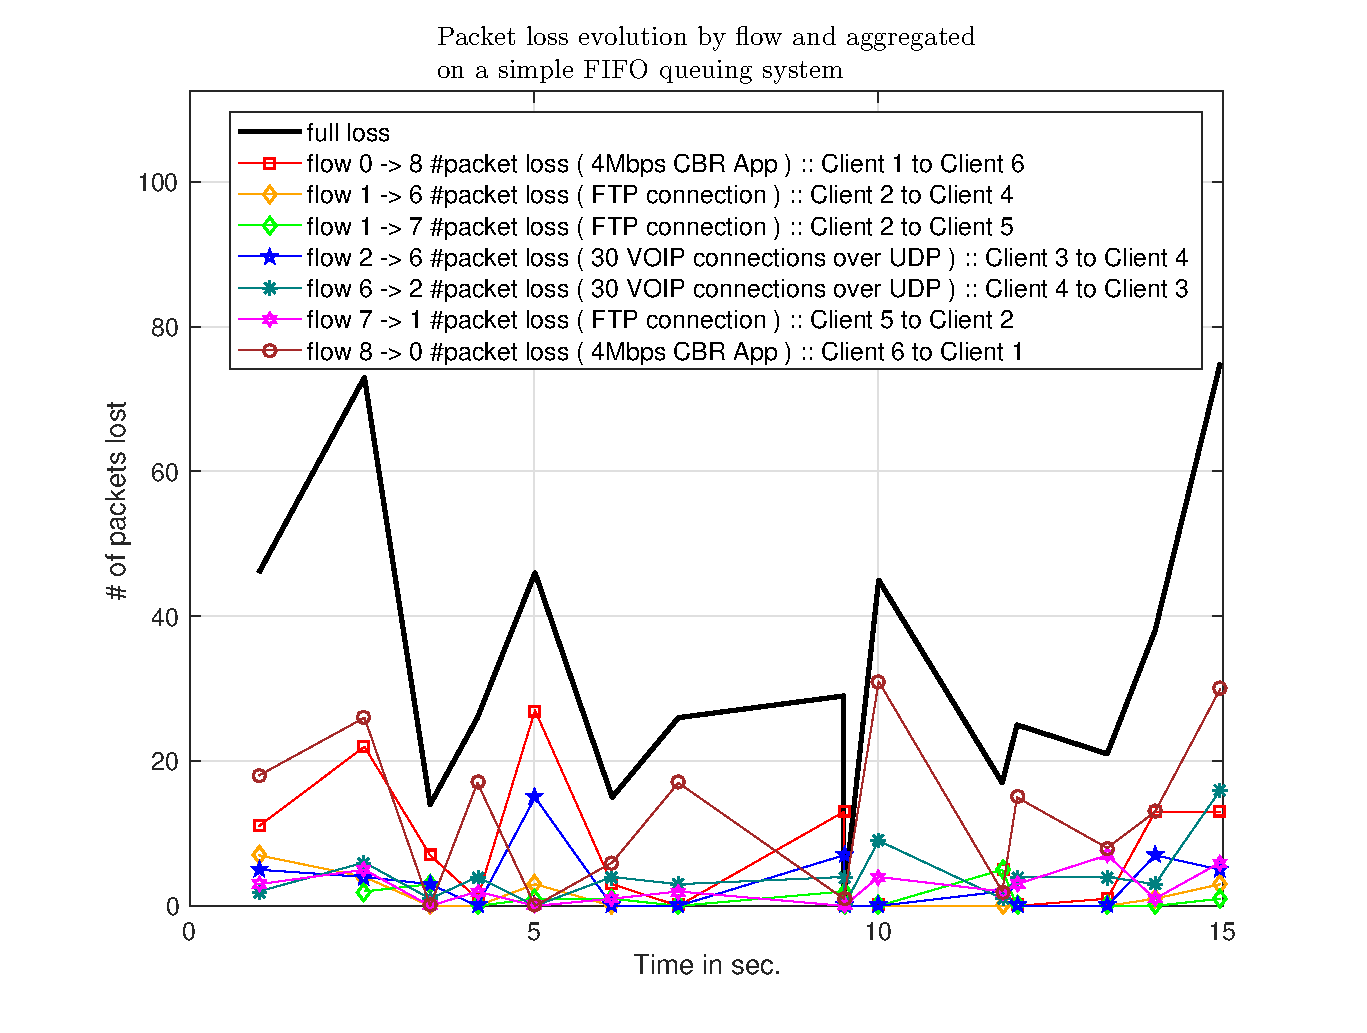
\includegraphics[width=1\columnwidth]{EPS/B/loss_b1.eps}
     \caption{Packet loss evolution by flow and aggregated on a simple FIFO queueing system, simulating a multi-service network in a "best effort" scenario.}
     \label{graph:loss_b11}
     \end{figure}

     As you can state in figure \ref{graph:loss_b11}, services like VOIP connections over UDP and FTP connections suffer the most when the network is fully congested, being the flows 1 $ \rightarrow $ 7 ( FTP connection ), 2 $ \rightarrow $ 6 ( 30 VOIP connections over UDP ),  and  6 $ \rightarrow $ 2 ( 30 VOIP connections over UDP ), the ones that are most affected. \par 
     The relation between flow, total number of packets lost, and percentage of loss/sent packages, is presented in table \ref{table:loss_b1}, and lets us fully understand the harm of treating all traffic with the same priority.\par 



     \begin{table}[H]
     \caption{Relation between flow, total number of packets lost, total number of packets sent, and percentage of loss/sent packages, on a simple FIFO queueing system, simulating a multi-service network in a "best effort" scenario.}
     \label{table:loss_b1}
     \centering
     \begin{tabular}{ | L{3.5cm} | R{1.0cm} | R{1.0cm} | R {1.2  cm} |}
     \hline  Flow & \#packets loss &  \#packets received  & \% loss/received  \\ \hline \hline
     \tiny{ 0 $ \rightarrow $ 8 ( 4 Mbps CBR App )}  &    116   &  29652  & 0.3912 \% \\ \hline
     \tiny{ 1 $ \rightarrow $ 6 ( FTP connection )} &    20   &  3720  &  0.5376 \% \\ \hline
     \tiny{1 $ \rightarrow $ 7 ( FTP connection )} &    15   &   3743 & 0.4007 \% \\ \hline
     \tiny{  2 $ \rightarrow $ 6 ( 30 VOIP connections over UDP )} &    48   &   4016  & 1.1952 \% \\ \hline
     \tiny{    6 $ \rightarrow $ 2 ( 30 VOIP connections over UDP )} &    61   &   4349  & 1.4026 \% \\ \hline
     \tiny{  7 $ \rightarrow $ 1 ( FTP connection )} &    36   &   3620 & 0.9945 \% \\ \hline
     \tiny{ 8 $ \rightarrow $ 0 ( 4 Mbps CBR App )} &    185   &    29445 & 0.6283 \% \\ \hline
     \end{tabular}
     \end{table}

     Please denote that despite the loss percentage doesn't seem to high for all flows, those values are presented as a mean value, giving the possibility of loss increase in certain time intervals, and decrease in others. We should therefore analyse the percentage of loss per flow by connection time.  The corresponding results are shown in figure \ref{graph:loss_sent_percentage_b1}.

     \begin{figure}[H]
     \centering
     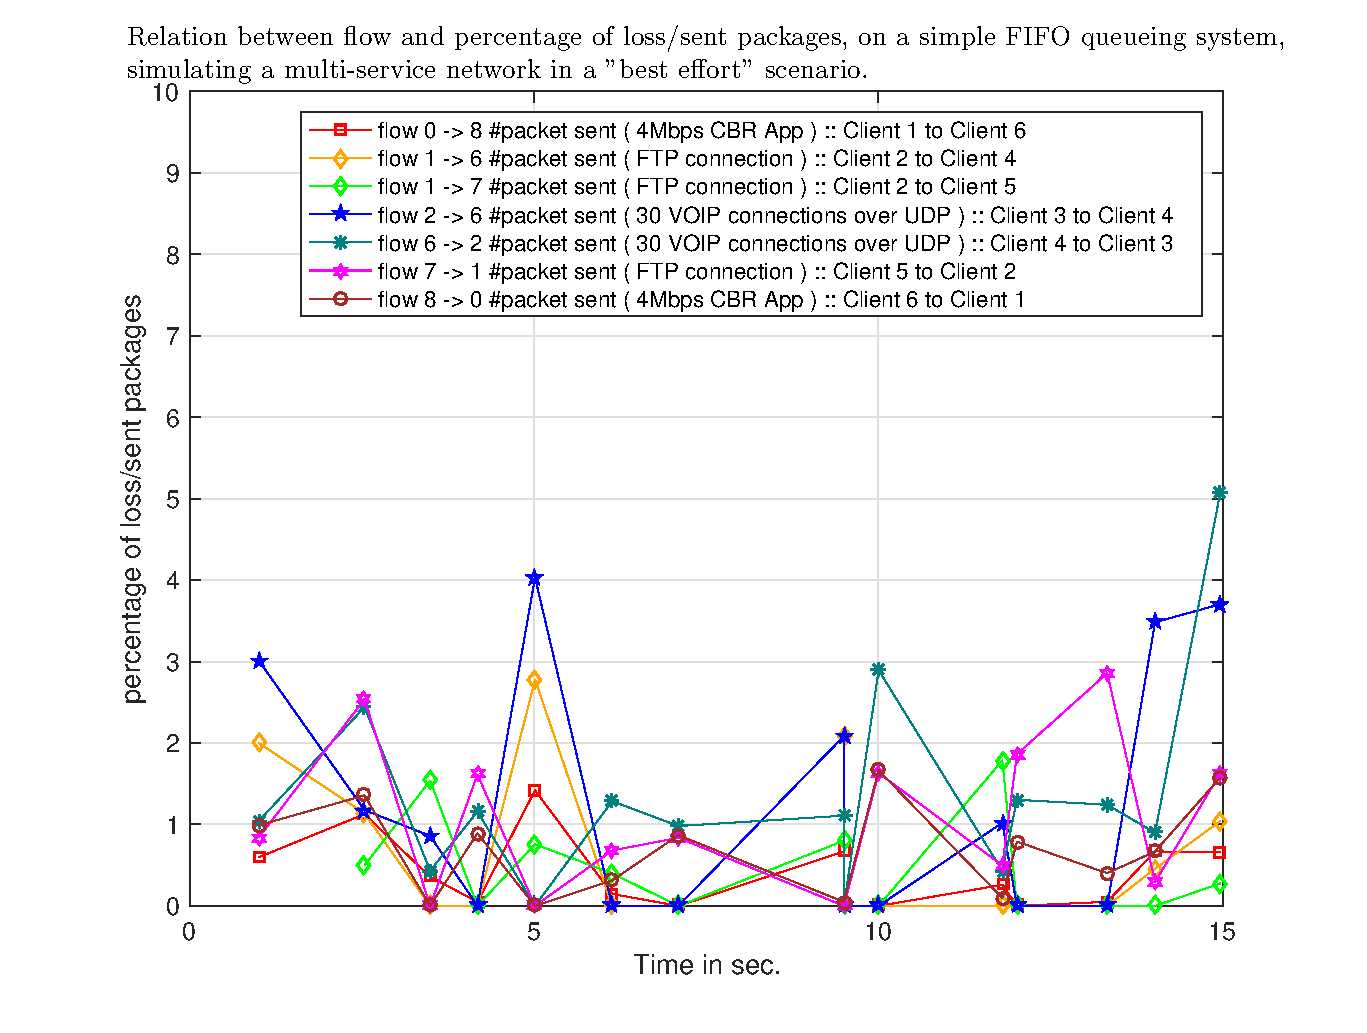
\includegraphics[width=1\columnwidth]{EPS/B/loss_sent_percentage_b1.eps}
     \caption{Packet loss/sent percentage by flow evolution, on a simple FIFO queueing system, simulating a multi-service network in a "best effort" scenario.}
     \label{graph:loss_sent_percentage_b1}
     \end{figure}


     As stated before, it is in flows 2 $ \rightarrow $ 6 ( 30 VOIP connections over UDP ) and 6 $ \rightarrow $ 2 ( 30 VOIP connections over UDP ) that we observe a bigger loss percentage over time (5\%). The service that should be prioritised and treated as the most volatile to delays (real time traffic necessity) is the one suffering the most from congestion. 

\section{Simulating Differentiated Services :: protecting vulnerable packets}
\label{diffserv}
In some flows, the loss of some segments has more impact than others on the perfomance of the service/application -- as FTP (over TCP) and VOIP (over UDP). We call the packets from these services, our vulnerable packets in our simulation scenario. By "marking" these segments/packets with a higher priority and implementing the priority using a diffserv architecture, the overall perfomance and QoS considerably improves. \par 
For a first approach we considered similar clients with CBR applications,  generating each one a rate of 3Mbps, for a total of six flows (0 $ \rightarrow $ 8, 1 $ \rightarrow $ 7, 2 $ \rightarrow $ 6, 8 $ \rightarrow $0, 7 $ \rightarrow $1,    6 $ \rightarrow $2).\par 
We considered the simple network topology defined in figure \ref{fig:network}, and before any further change we analysed the links under congestion, and identified the queue which suffers higher packet
loss.\par 

     \subsection{Identification of the queueing management parameters for an Edge $\rightarrow$  Core Configuration and an Core $\rightarrow$  Edge Configuration}
     
     The presented parameters for an Edge $\rightarrow$  Core Configuration and an Core $\rightarrow$  Edge Configuration, were not chosen to necessarily obtain an optimal initial performance, but rather to create conditions that allow us to study the effect of diffserv on diminishing the loss probabilities of vulnerable flows, and the impact of the further changes versus this initial simple configuration.\par 
     
     Consider this simulation scenario and its initial traffic model as a base comparison model for the "best-effort" model presented in section \ref{besteffort} on page \pageref{besteffort}.

     \subsubsection{E1 - C0 (Edge $\rightarrow$ Core Configuration)}
     \begin{itemize}
     \item \textbf{The number of existing queues and the traffic scheduler in use} \par 
     1 physical queue,  implementing 2 virtual queues;  
     \vspace{5mm}
     \item \textbf{Policy Entry}
     \begin{itemize}
     \item \textbf{Client1 $\rightarrow$ Client6} -- TokenBucket:
     \begin{itemize}
     \item \textbf{Committed Information Rate:} 2 Mbits/sec;
     \item \textbf{Committed Burst Size:} 5 KBytes;
     \item \textbf{Policer Table} has initial (green) code point 10, and downgraded (yellow) code point 11;
     \end{itemize}
     \item \textbf{Every remaining initial and end station} -- Dumb:
     \begin{itemize}
     \item \textbf{Policer Table} has always downgraded (yellow) code point 11;
     \end{itemize}
     \end{itemize}

     \vspace{5mm}
     \item \textbf{The queueing discipline in use and the configuration of each queue:}\par
     Round Robin scheduling and RIO-C Active Queue Management: \par 
     \begin{itemize}
     \item queue 0:
     \begin{itemize}
     \item \textbf{minimum threshold}: 20 Packets;
     \item \textbf{maximum threshold}: 40 Packets;
     \item \textbf{maximum dropping probability}: $2 * 10^{-2}$;
     \end{itemize}
     \item queue 1:
     \begin{itemize}
     \item \textbf{minimum threshold}: 10 Packets;
     \item \textbf{maximum threshold}: 20 Packets;
     \item \textbf{maximum dropping probability}:  $1 * 10^{-1}$;
     \end{itemize}
     \end{itemize}

     \vspace{5mm}
     \item \textbf{the amount of memory allocated to the queues:}\par

     Default queue buffer size is 20 packets (Packet size 1 KB) : 20KB per queue;


     \vspace{5mm}
     \item \textbf{the queues which handle data flows:}\par
     Code point 10 mapped to physical queue 0 and virtual queue 0, Code point 11 mapped to physical queue 0 and virtual queue 1;

     \end{itemize}


     \subsubsection{C0 - E2 (Core $\rightarrow$ Edge Configuration)}


     \begin{itemize}
     \item \textbf{The number of existing queues and the traffic scheduler in use} \par 
     1 physical queue,  implementing 2 virtual queues;  
     \vspace{5mm}

     \item \textbf{The queueing discipline in use and the configuration of each queue:}\par
     Round Robin scheduling and RIO-C Active Queue Management: \par 
     \begin{itemize}
     \item queue 0:
     \begin{itemize}
     \item \textbf{minimum threshold}: 20 Packets;
     \item \textbf{maximum threshold}: 40 Packets;
     \item \textbf{maximum dropping probability}: $2 * 10^{-2}$;
     \end{itemize}
     \item queue 1:
     \begin{itemize}
     \item \textbf{minimum threshold}: 10 Packets;
     \item \textbf{maximum threshold}: 20 Packets;
     \item \textbf{maximum dropping probability}:  $1 * 10^{-1}$;
     \end{itemize}
     \end{itemize}

     \vspace{5mm}
     \item \textbf{the amount of memory allocated to the queues:}\par

     Default queue buffer size is 20 packets (Packet size 1 KB) : 20KB per queue;


     \vspace{5mm}
     \item \textbf{the queues which handle data flows:}\par
     Code point 10 mapped to physical queue 0 and virtual queue 0, Code point 11 mapped to physical queue 0 and virtual queue 1;

     \end{itemize}

   \subsection{Identification of the queue which suffers higher packet loss}

Taking into account the simulation results/statistics, presented on tables \ref{table:e1_c0_5s} to \ref{table:c0_e2_15s}, we can identify the queue which suffers higher packet loss -- physical queue 0 and virtual queue 1, from E1 to C0 (Edge $\rightarrow$ Core Configuration). This behaviour is easily explained since every traffic with initial station that is not Client1, and end station that is not Client6, is always downgrade to code point 11 (yellow tag). In congestion, these are the first packets to be dropped (wether late dropped or early dropped).
\subsubsection{Statistics for time = 5s}
.
\begin{table}[H]
     \caption{Statistics for the queue from E1 to C0 (Edge $\rightarrow$ Core Configuration) }
     \label{table:e1_c0_5s}
     \centering
     \begin{tabular}{ | L{1cm} | R{1.0cm} | R{1.0cm} | R {1.0  cm} | R {1.0  cm} |}
     \hline  CP & TotPkts &  TxPkts  & ldrops &  edrops \\ \hline \hline
     
    All   &  5619   &  3136    & 2097  &    386 \\ \hline
 10   &  1252 &    1252    &    0  &      0\\ \hline
 11    & 4367    & 1884  &   2097   &   386\\ \hline
     \end{tabular}
     \end{table}

\begin{table}[H]
     \caption{Statistics for the queue from C0 to E2 (Core $\rightarrow$  Edge Configuration) }
     \label{table:c0_e2_5s}
     \centering
     \begin{tabular}{ | L{1cm} | R{1.0cm} | R{1.0cm} | R {1.0  cm} | R {1.0  cm} |}
     \hline  CP & TotPkts &  TxPkts  & ldrops &  edrops \\ \hline \hline
    All   &  3111   &  3111    & 0  &    0 \\ \hline
 10   &  1242 &    1242    &    0  &      0\\ \hline
 11    & 1869    & 1869  &   0   &   0\\ \hline
     \end{tabular}
     \end{table}
     
 
 
 \subsubsection{Statistics for time = 10s}
.
\begin{table}[H]
     \caption{Statistics for the queue from E1 to C0 (Edge $\rightarrow$ Core Configuration) }
     \label{table:e1_c0_10s}
     \centering
     \begin{tabular}{ | L{1cm} | R{1.0cm} | R{1.0cm} | R {1.0  cm} | R {1.0  cm} |}
     \hline  CP & TotPkts &  TxPkts  & ldrops &  edrops \\ \hline \hline
     
    All   &  11244   &  6261    & 4197  &    786 \\ \hline
 10   &  2502 &    2502    &    0  &      0\\ \hline
 11    & 8742    & 3759  &   4197   &   786\\ \hline
     \end{tabular}
     \end{table}

\begin{table}[H]
     \caption{Statistics for the queue from C0 to E2 (Core $\rightarrow$  Edge Configuration) }
     \label{table:c0_e2_10s}
     \centering
     \begin{tabular}{ | L{1cm} | R{1.0cm} | R{1.0cm} | R {1.0  cm} | R {1.0  cm} |}
     \hline  CP & TotPkts &  TxPkts  & ldrops &  edrops \\ \hline \hline
    All   &  6236   &  6236    & 0  &    0 \\ \hline
 10   &  2492 &    2492    &    0  &      0\\ \hline
 11    & 3744    & 3744  &   0   &   0\\ \hline
     \end{tabular}
     \end{table}
     
 

 \subsubsection{Statistics for time = 15s}
.

\begin{table}[H]
     \caption{Statistics for the queue from E1 to C0 (Edge $\rightarrow$ Core Configuration) }
     \label{table:e1_c0_15s}
     \centering
     \begin{tabular}{ | L{1cm} | R{1.0cm} | R{1.0cm} | R {1.0  cm} | R {1.0  cm} |}
     \hline  CP & TotPkts &  TxPkts  & ldrops &  edrops \\ \hline \hline
     
    All   &  16869   &  9386    & 6298  &    1185 \\ \hline
 10   &  3752 &    3752    &    0  &      0\\ \hline
 11    & 13117    & 5634  &   6298   &   1185\\ \hline
     \end{tabular}
     \end{table}
 
 
\begin{table}[H]
     \caption{Statistics for the queue from C0 to E2 (Core $\rightarrow$  Edge Configuration) }
     \label{table:c0_e2_15s}
     \centering
     \begin{tabular}{ | L{1cm} | R{1.0cm} | R{1.0cm} | R {1.0  cm} | R {1.0  cm} |}
     \hline  CP & TotPkts &  TxPkts  & ldrops &  edrops \\ \hline \hline
    All   &  9361   &  9361    & 0  &    0 \\ \hline
 10   &  3742 &    3742    &    0  &      0\\ \hline
 11    & 5619    & 5619  &   0   &   0\\ \hline
     \end{tabular}
     \end{table}
     
\subsection{A visual interpretation of the packet loss and bandwidth utilisation along the time}

Given the simulation scenario and the initial traffic model presented on section \ref{diffserv} on page \pageref{diffserv}, the corresponding results illustration the levels of loss and bandwidth utilisation along time are show in figures \ref{graph:bw_c3} and \ref{graph:loss_c3}.

  \begin{figure}[H]
     \centering
     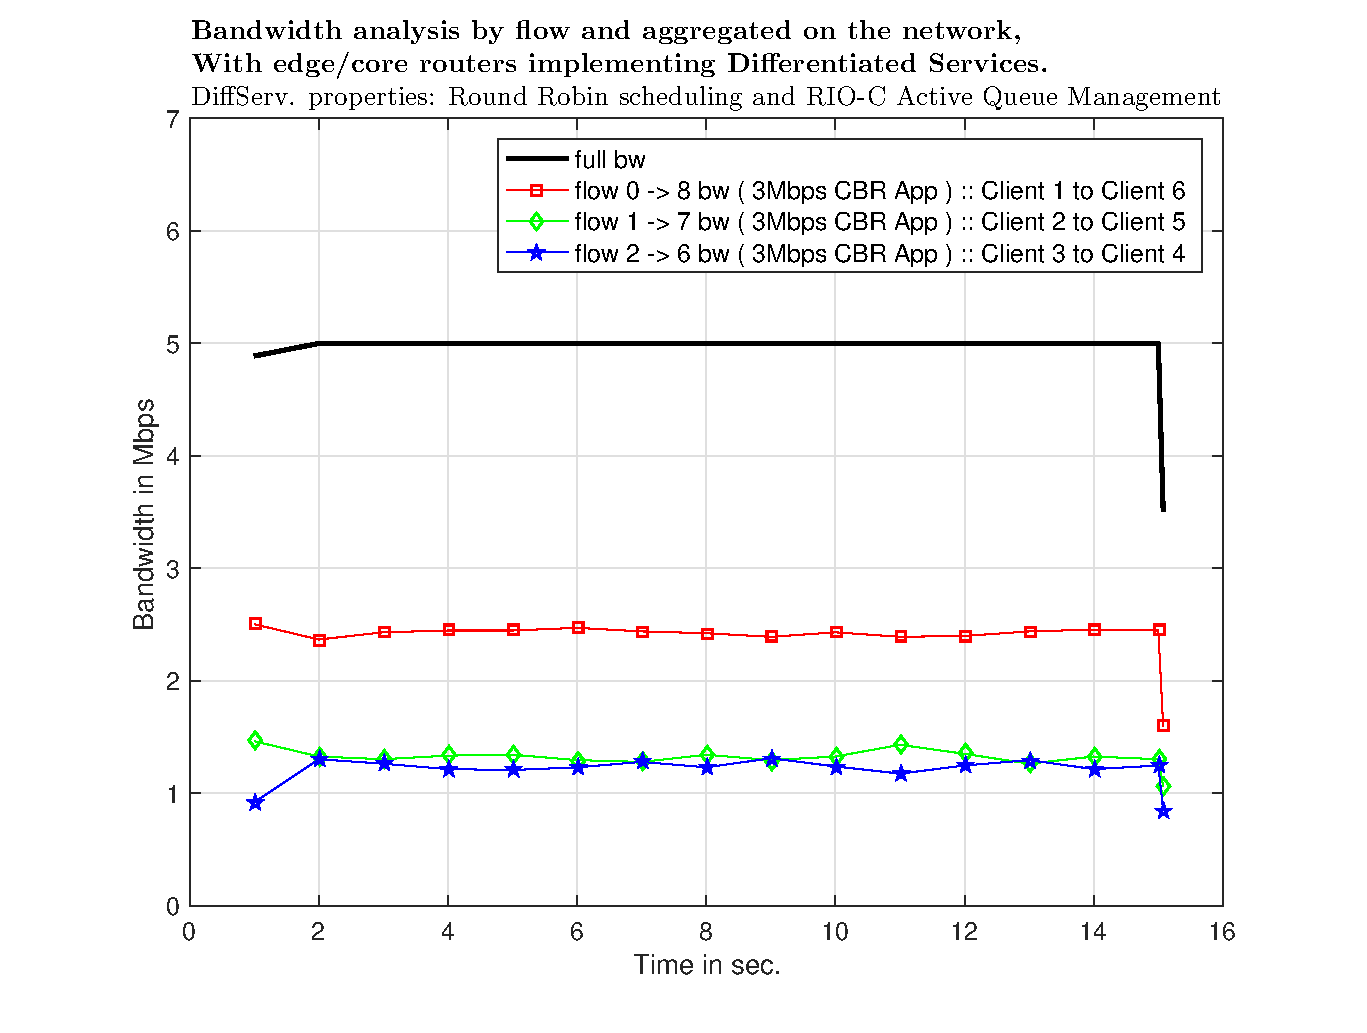
\includegraphics[width=1\columnwidth]{EPS/C/bw_c3.eps}
     \caption{Bandwidth analysis by flow and aggregated on a simple FIFO queueing system, using Random Early Detection Gateways for congestion avoidance.}
     \label{graph:bw_c3}
     \end{figure}


     \begin{figure}[H]
     \centering
     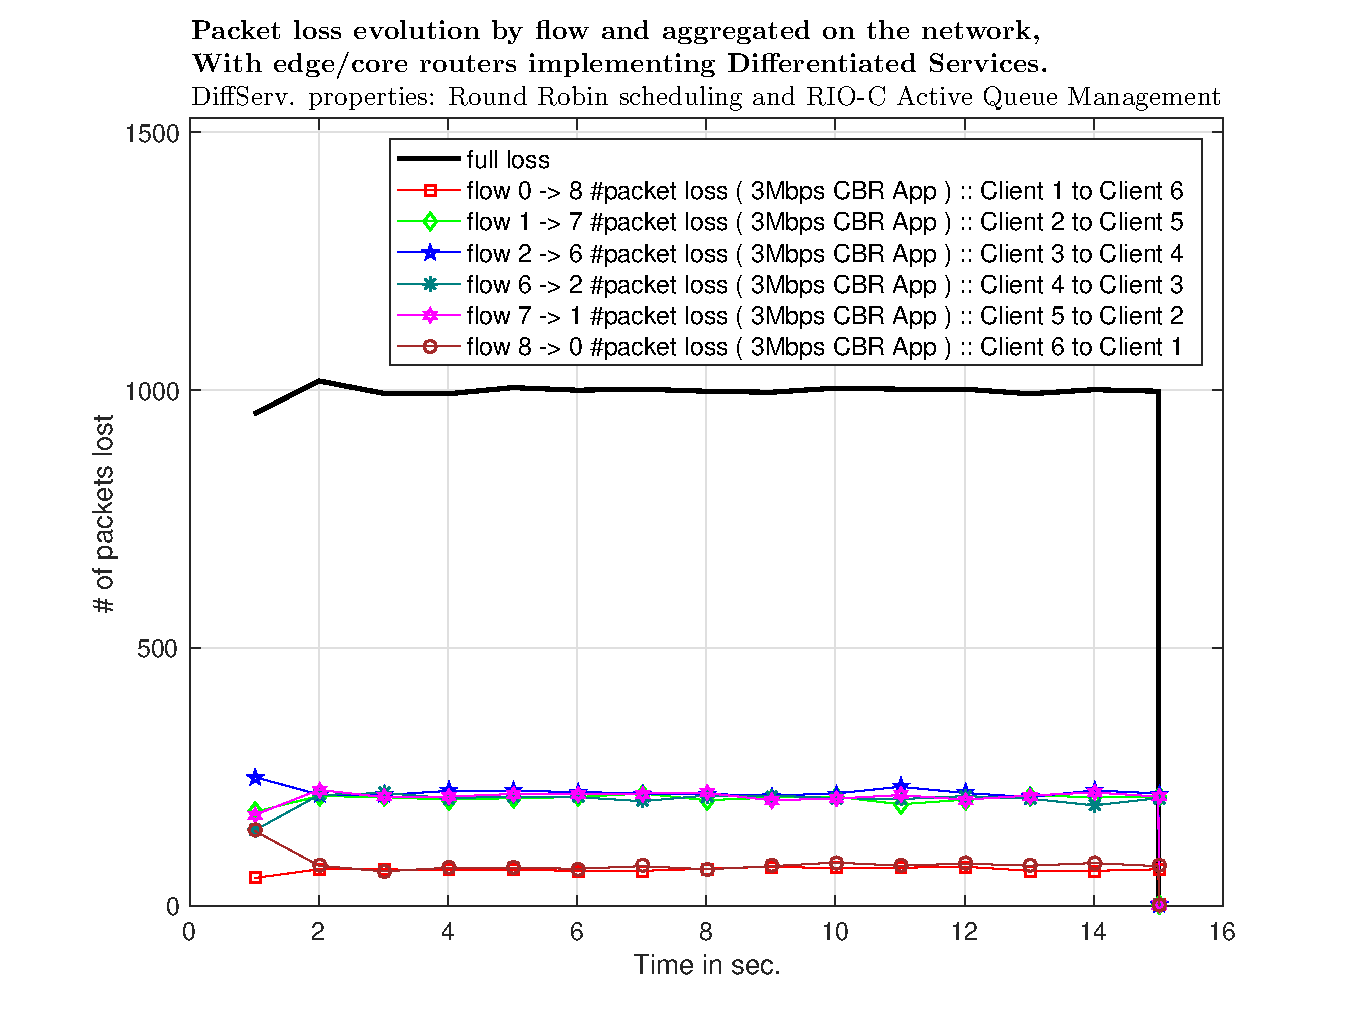
\includegraphics[width=1\columnwidth]{EPS/C/loss_c3.eps}
     \caption{Packet loss evolution by flow and aggregated on a simple FIFO queueing system, using Random Early Detection Gateways for congestion avoidance.}
     \label{graph:loss_c3}
     \end{figure}

When comparing the simulation results to the "best-effort" scenario we conclude that, despite the "final solution" being unacceptable, every flow obtains some quota of the available total bandwidth. We can observe that we also achieved a better packet loss maximum for all the simulation flows (approximately 250 vs 400 for the "best-effort" scenario). We have achived differentiated services for th
e same type of traffic, based on the initial station and end station of every traffic. \par
Given that, the next step is to assume that traffic from all clients is marked as belonging to the same class of service, and verify if the option for a single traffic class bring any added value to network QoS when compared with the best-effort scenario. 
The corresponding results are shown in figures \ref{graph:bw_c4} and \ref{graph:loss_c4}.


\begin{figure}[H]
     \centering
     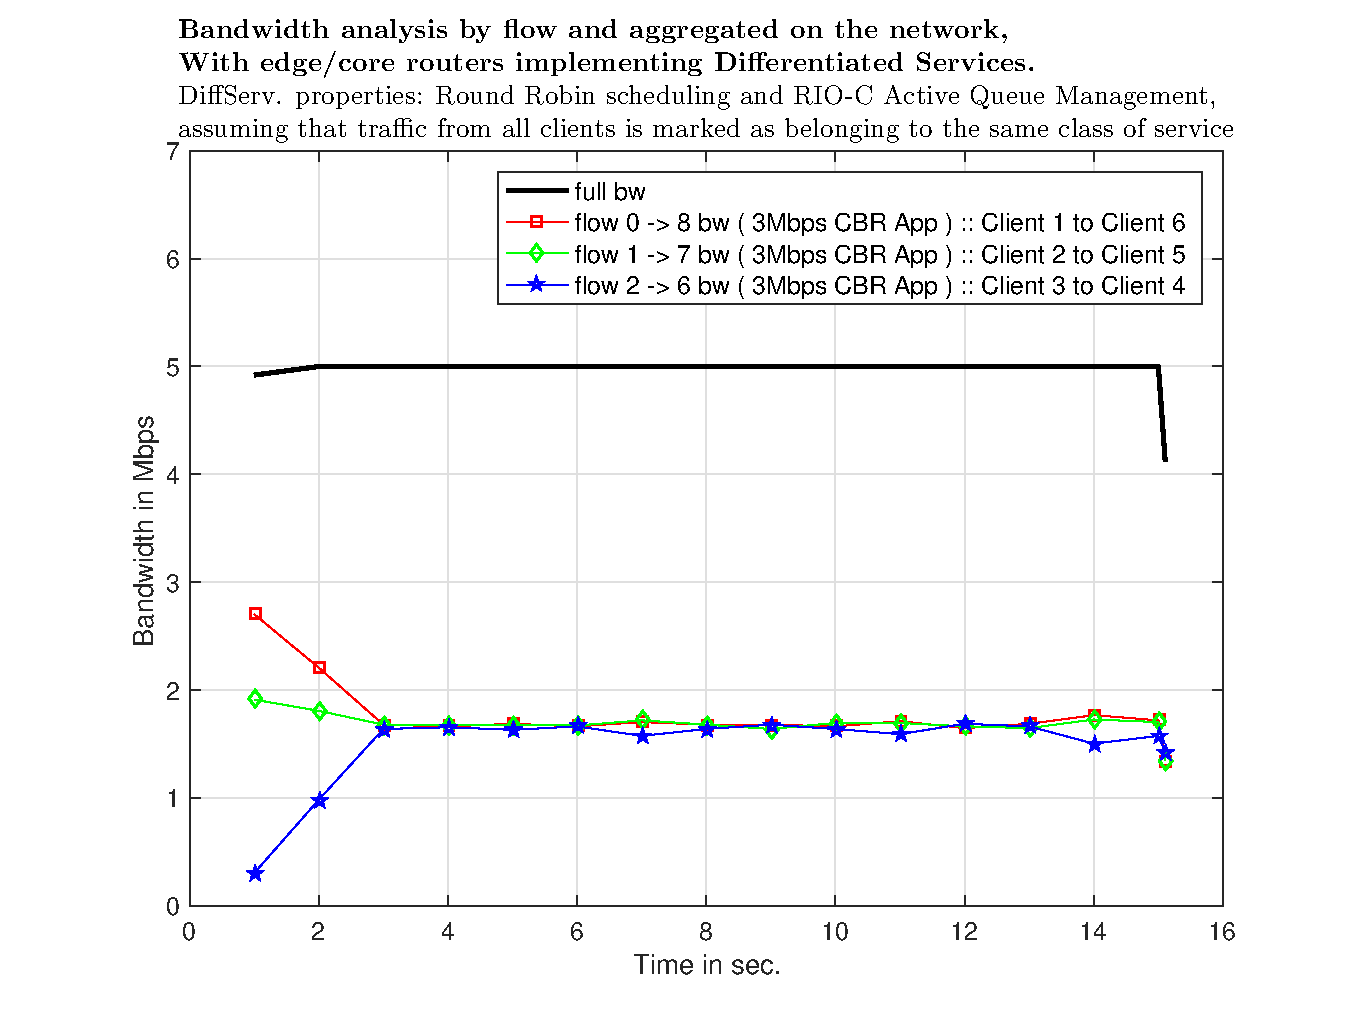
\includegraphics[width=1\columnwidth]{EPS/C/bw_c4.eps}
     \caption{Bandwidth analysis by flow and aggregated on a simple FIFO queueing system, using Random Early Detection Gateways for congestion avoidance.}
     \label{graph:bw_c4}
     \end{figure}


     \begin{figure}[H]
     \centering
     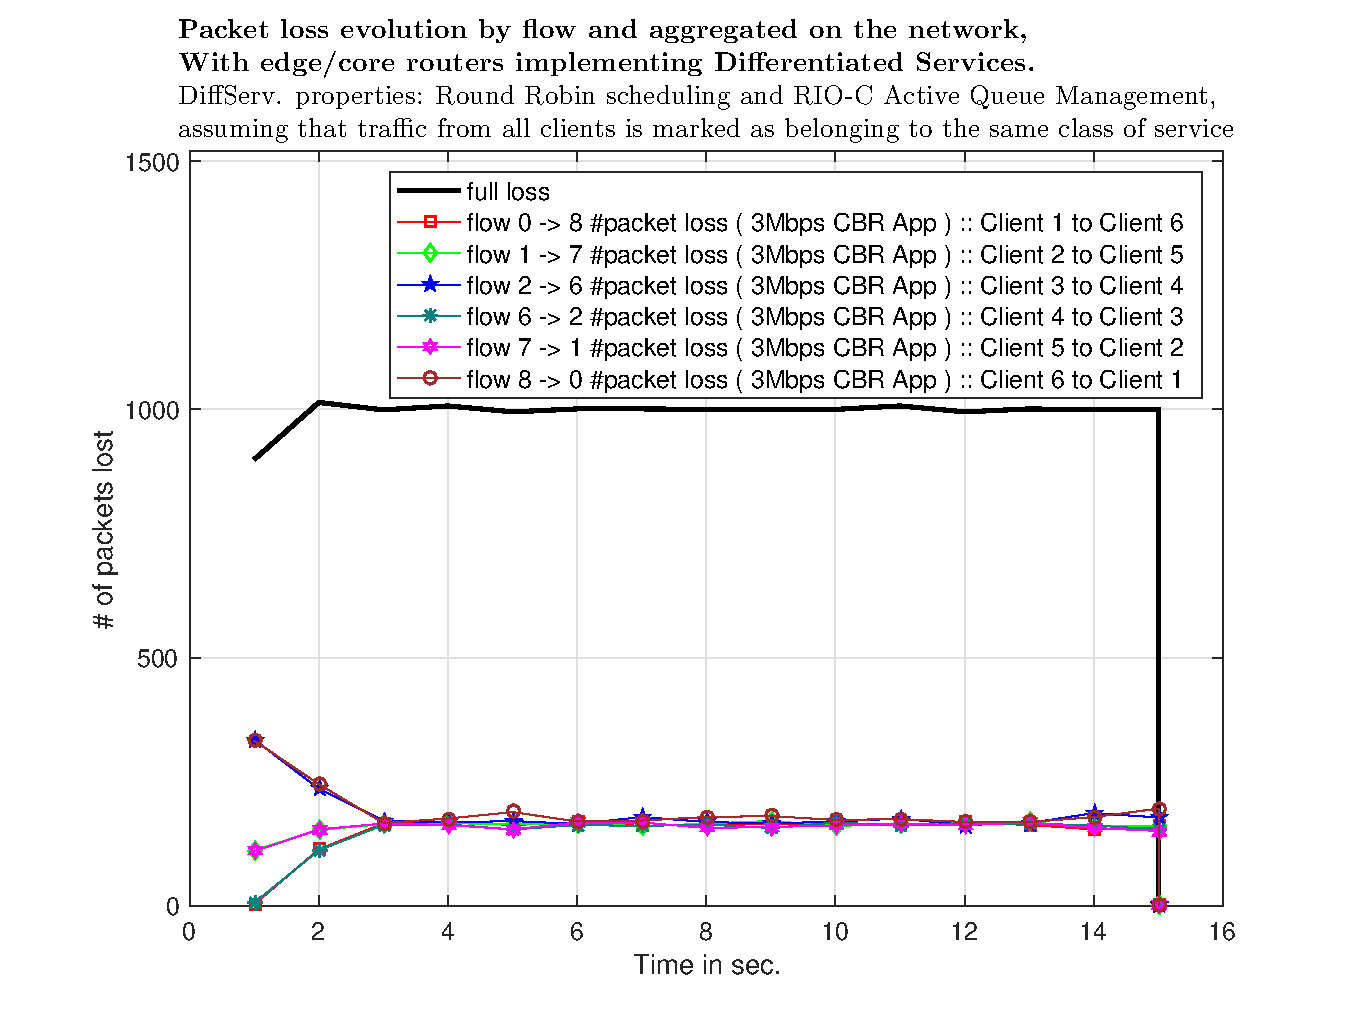
\includegraphics[width=1\columnwidth]{EPS/C/loss_c4.eps}
     \caption{Packet loss evolution by flow and aggregated on a simple FIFO queueing system, using Random Early Detection Gateways for congestion avoidance.}
     \label{graph:loss_c4}
     \end{figure}

     Notice that this "solution" only improves the equitable bandwidth distribution across flow because they all are produced with the same service/traffic type, and, when compared to the "best-effort" scenario with Random Early Detection for Congestion Avoidance, the only improvement is the possibility of limiting the bandwidth percentage to be used, since we can "become" harsher to the yellow tagged traffic increasing its maximum dropping probability to 1, and therefore dropping every traffic out the Committed Information Rate limit. \par
     But the problem of the multi-services in the network maintains. In this simple simulation scenario there is only the possibility of tagging traffic to be "in-bounds" or "out-of-bounds". If we added both UDP and TCP traffic with other characteristics, the problems identified in section \ref{multiservice} would still be observed.
     
     
 \subsection{Simulating a multi-service network in a DiffServ scenario}
  Suppose that the service provider intends to implement the following policy:
  \begin{itemize}
  \item To assure a 30 \% of capacity to clients with identical characteristics (the full capacity may be
used if available).
  \item Traffic exceeding the negotiated rate must be downgraded, i.e., forwarded with lower priority.
  \end{itemize}
  Using the procedures already included in the simulation script, several changes were made in order to obtain the following traffic model:
   \begin{itemize}
     \item a \textbf{CBR application} sending 4Mbps from client 1 to client 6, starting at 2.5s;
          \item a \textbf{CBR application} sending 4Mbps from client 2 to client 4, starting at 5s;
          \item a \textbf{CBR application} sending 4Mbps from client 5 to client 2, starting at 10s;
              \item a \textbf{CBR application} sending 4Mbps from client 6 to client 1, starting at 0s;
     \item  a \textbf{FTP connection} from client 2 to client 5, and other from client 4 to client 2;
     \item  a \textbf{voice connection over UDP} from client 3 to client 4, and vice-versa. Since VOIP Bandwidth consumption naturally depends on the codec used, we selected G.711 - 64 Kbps Bitrate and 87.2 Kbps Nominal Ethernet Bandwidth, and simulated a maximum of 30 calls at any given simulation time. The presented graphic results for VOIP are an aggregation of all the 30 calls. 
     \end{itemize}
\par 
In order to correctly simulate Differentiated Services, giving special attention in protecting vulnerable real-time packets, several changes were made to the parameters for  Edge $\rightarrow$  Core Configurations and an Core $\rightarrow$  Edge Configurations:


     \subsubsection{Edge $\rightarrow$ Core Configurations}
     \begin{itemize}
     \item \textbf{The number of existing queues and the traffic scheduler in use} \par 
     3 physical queues, each implementing 3 virtual queues;  
     \vspace{5mm}
     \item \textbf{Policy Entry}
     \begin{itemize}
     
    	 \item \textbf{Client1 $\rightarrow$ Client6  ( 4 Mbps CBR App )} -- Two Rate Three Color Marker:
   	  	\begin{itemize}
   	 	 \item \textbf{Committed Information Rate:} 1 Mbits/sec;
   		  \item \textbf{Committed Burst Size:} 5 KBytes;
		    \item \textbf{Peak Information Rate:} 3 Mbits/sec;
		     \item \textbf{Peak Burst Size:} 5 KBytes;
  		   \item \textbf{Policer Table} has initial (green) code point 10, and downgraded (yellow) code point 11, and further downgraded (red) code point 12;
     		\end{itemize}
		
		\item \textbf{Client2 $\rightarrow$ Client4  ( 4 Mbps CBR App )} -- Two Rate Three Color Marker:
   	  	\begin{itemize}
   	 	 \item \textbf{Committed Information Rate:} 1 Mbits/sec;
   		  \item \textbf{Committed Burst Size:} 5 KBytes;
		    \item \textbf{Peak Information Rate:} 3 Mbits/sec;
		     \item \textbf{Peak Burst Size:} 5 KBytes;
  		   \item \textbf{Policer Table} has initial (green) code point 10, and downgraded (yellow) code point 11, and further downgraded (red) code point 12;
     		\end{itemize}
		
		
		\item \textbf{Client2 $\rightarrow$ Client5  ( FTP connection )} -- Time Sliding Window Three Color Marker:
   	  	\begin{itemize}
   	 	 \item \textbf{Committed Information Rate:} 1 Mbits/sec;
		    \item \textbf{Peak Information Rate:} 3 Mbits/sec;
  		   \item \textbf{Policer Table} has initial (green) code point 7, and downgraded (yellow) code point 8, and further downgraded (red) code point 9;
     		\end{itemize}
		
		
		
		
		\item \textbf{Client3 $\rightarrow$ Client4 ( 30 VOIP connections over UDP )} -- TokenBucket:
   	  	\begin{itemize}
   	 	 \item \textbf{Committed Information Rate:} 1 Mbits/sec;
   		  \item \textbf{Committed Burst Size:} 5 KBytes;
  		   \item \textbf{Policer Table} has initial (green) code point 4, and downgraded (yellow) code point 5;
     		\end{itemize}

\item \textbf{Client4 $\rightarrow$ Client2  ( FTP connection )} -- Time Sliding Window Three Color Marker:
   	  	\begin{itemize}
   	 	 \item \textbf{Committed Information Rate:} 1 Mbits/sec;
		    \item \textbf{Peak Information Rate:} 3 Mbits/sec;
  		   \item \textbf{Policer Table} has initial (green) code point 7, and downgraded (yellow) code point 8, and further downgraded (red) code point 9;
     		\end{itemize}
		
		\item \textbf{Client4 $\rightarrow$ Client3 ( 30 VOIP connections over UDP )} -- TokenBucket:
   	  	\begin{itemize}
   	 	 \item \textbf{Committed Information Rate:} 1 Mbits/sec;
   		  \item \textbf{Committed Burst Size:} 5 KBytes;
  		   \item \textbf{Policer Table} has initial (green) code point 4, and downgraded (yellow) code point 5;
     		\end{itemize}
		

	\item \textbf{Client5 $\rightarrow$ Client2  ( 4 Mbps CBR App )} -- Two Rate Three Color Marker:
   	  	\begin{itemize}
   	 	 \item \textbf{Committed Information Rate:} 1 Mbits/sec;
   		  \item \textbf{Committed Burst Size:} 5 KBytes;
		    \item \textbf{Peak Information Rate:} 3 Mbits/sec;
		     \item \textbf{Peak Burst Size:} 5 KBytes;
  		   \item \textbf{Policer Table} has initial (green) code point 10, and downgraded (yellow) code point 11, and further downgraded (red) code point 12;
     		\end{itemize}
		
			\item \textbf{Client6 $\rightarrow$ Client1  ( 4 Mbps CBR App )} -- Two Rate Three Color Marker:
   	  	\begin{itemize}
   	 	 \item \textbf{Committed Information Rate:} 1 Mbits/sec;
   		  \item \textbf{Committed Burst Size:} 5 KBytes;
		    \item \textbf{Peak Information Rate:} 3 Mbits/sec;
		     \item \textbf{Peak Burst Size:} 5 KBytes;
  		   \item \textbf{Policer Table} has initial (green) code point 10, and downgraded (yellow) code point 11, and further downgraded (red) code point 12;
     		\end{itemize}
     
     \item \textbf{Every remaining initial and end station} -- Dumb:
     \begin{itemize}
     \item \textbf{Policer Table} has always downgraded (yellow) code point 11;
     \end{itemize}
     \end{itemize}

     \vspace{5mm}
     \item \textbf{The queueing discipline in use and the configuration of each queue:}\par
     Weighted Round Robin scheduling and RIO-C Active Queue Management: \par 
     \begin{itemize}
     \item physical queue 0:
     \begin{itemize}
     	\item virtual queue 0:
     	\begin{itemize}
     		\item \textbf{minimum threshold}: 20 Packets;
		     \item \textbf{maximum threshold}: 40 Packets;
		     \item \textbf{maximum dropping probability}: $2 * 10^{-2}$;
         \end{itemize}
    	 \item virtual queue 1:
   	  \begin{itemize}
     			\item \textbf{minimum threshold}: 10 Packets;
 			    \item \textbf{maximum threshold}: 20 Packets;
   			  \item \textbf{maximum dropping probability}: $1 * 10^{-1}$;
  	   \end{itemize}
	   
	   \item virtual queue 2:
   	  \begin{itemize}
     			\item \textbf{minimum threshold}: 5 Packets;
 			    \item \textbf{maximum threshold}: 10 Packets;
   			  \item \textbf{maximum dropping probability}: $5 * 10^{-1}$;
  	   \end{itemize}   
    \end{itemize}
    
    
      \item physical queue 1:
     \begin{itemize}
     	\item virtual queue 0:
     	\begin{itemize}
     		\item \textbf{minimum threshold}: 10 Packets;
		     \item \textbf{maximum threshold}: 20 Packets;
		     \item \textbf{maximum dropping probability}: $2 * 10^{-2}$;
         \end{itemize}
    	 \item virtual queue 1:
   	  \begin{itemize}
     			\item \textbf{minimum threshold}: 5 Packets;
 			    \item \textbf{maximum threshold}: 10 Packets;
   			  \item \textbf{maximum dropping probability}: $1 * 10^{-1}$;
  	   \end{itemize}
	   
	   \item virtual queue 2:
   	  \begin{itemize}
     			\item \textbf{minimum threshold}: 1 Packets;
 			    \item \textbf{maximum threshold}: 5 Packets;
   			  \item \textbf{maximum dropping probability}: $5 * 10^{-1}$;
  	   \end{itemize}   
    \end{itemize}


  \item physical queue 2:
     \begin{itemize}
     	\item virtual queue 0:
     	\begin{itemize}
     		\item \textbf{minimum threshold}: 10 Packets;
		     \item \textbf{maximum threshold}: 20 Packets;
		     \item \textbf{maximum dropping probability}: $2 * 10^{-2}$;
         \end{itemize}
    	 \item virtual queue 1:
   	  \begin{itemize}
     			\item \textbf{minimum threshold}: 5 Packets;
 			    \item \textbf{maximum threshold}: 10 Packets;
   			  \item \textbf{maximum dropping probability}: $1 * 10^{-1}$;
  	   \end{itemize}
	   
	   \item virtual queue 2:
   	  \begin{itemize}
     			\item \textbf{minimum threshold}: 1 Packets;
 			    \item \textbf{maximum threshold}: 5 Packets;
   			  \item \textbf{maximum dropping probability}: 1;
  	   \end{itemize}   
    \end{itemize}

     
     \end{itemize}

     \vspace{5mm}
     \item \textbf{the amount of memory allocated to the queues:}\par

     Default queue buffer size is 20 packets (Packet size 1 KB) : 20KB per queue;


     \vspace{5mm}
     \item \textbf{the queues which handle data flows:}\par
     \begin{itemize}
     \item \textbf{Code point 4}: mapped to physical queue 0 and virtual queue 0;
     \item \textbf{Code point 5}: mapped to physical queue 0 and virtual queue 1;
          
     \item \textbf{Code point 7}: mapped to physical queue 1 and virtual queue 0;
     \item \textbf{Code point 8}: mapped to physical queue 1 and virtual queue 1;
     \item \textbf{Code point 9}: mapped to physical queue 1 and virtual queue 2;

     \item \textbf{Code point 10}: mapped to physical queue 2 and virtual queue 0;
     \item \textbf{Code point 11}: mapped to physical queue 2 and virtual queue 1;
     \item \textbf{Code point 12}: mapped to physical queue 2 and virtual queue 2;


     \end{itemize}


     \end{itemize}


     \subsubsection{Core $\rightarrow$ Edge Configurations}


\begin{itemize}
     \item \textbf{The number of existing queues and the traffic scheduler in use} \par 
     3 physical queues, each implementing 3 virtual queues;  
     

     \vspace{5mm}
     \item \textbf{The queueing discipline in use and the configuration of each queue:}\par
     Weighted Round Robin scheduling and RIO-C Active Queue Management: \par 
     \begin{itemize}
     \item physical queue 0:
     \begin{itemize}
     	\item virtual queue 0:
     	\begin{itemize}
     		\item \textbf{minimum threshold}: 20 Packets;
		     \item \textbf{maximum threshold}: 40 Packets;
		     \item \textbf{maximum dropping probability}: $2 * 10^{-2}$;
         \end{itemize}
    	 \item virtual queue 1:
   	  \begin{itemize}
     			\item \textbf{minimum threshold}: 10 Packets;
 			    \item \textbf{maximum threshold}: 20 Packets;
   			  \item \textbf{maximum dropping probability}: $1 * 10^{-1}$;
  	   \end{itemize}
	   
	   \item virtual queue 2:
   	  \begin{itemize}
     			\item \textbf{minimum threshold}: 5 Packets;
 			    \item \textbf{maximum threshold}: 10 Packets;
   			  \item \textbf{maximum dropping probability}: $5 * 10^{-1}$;
  	   \end{itemize}   
    \end{itemize}
    
    
      \item physical queue 1:
     \begin{itemize}
     	\item virtual queue 0:
     	\begin{itemize}
     		\item \textbf{minimum threshold}: 10 Packets;
		     \item \textbf{maximum threshold}: 20 Packets;
		     \item \textbf{maximum dropping probability}: $2 * 10^{-2}$;
         \end{itemize}
    	 \item virtual queue 1:
   	  \begin{itemize}
     			\item \textbf{minimum threshold}: 5 Packets;
 			    \item \textbf{maximum threshold}: 10 Packets;
   			  \item \textbf{maximum dropping probability}: $1 * 10^{-1}$;
  	   \end{itemize}
	   
	   \item virtual queue 2:
   	  \begin{itemize}
     			\item \textbf{minimum threshold}: 1 Packets;
 			    \item \textbf{maximum threshold}: 5 Packets;
   			  \item \textbf{maximum dropping probability}: $5 * 10^{-1}$;
  	   \end{itemize}   
    \end{itemize}


  \item physical queue 2:
     \begin{itemize}
     	\item virtual queue 0:
     	\begin{itemize}
     		\item \textbf{minimum threshold}: 10 Packets;
		     \item \textbf{maximum threshold}: 20 Packets;
		     \item \textbf{maximum dropping probability}: $2 * 10^{-2}$;
         \end{itemize}
    	 \item virtual queue 1:
   	  \begin{itemize}
     			\item \textbf{minimum threshold}: 5 Packets;
 			    \item \textbf{maximum threshold}: 10 Packets;
   			  \item \textbf{maximum dropping probability}: $1 * 10^{-1}$;
  	   \end{itemize}
	   
	   \item virtual queue 2:
   	  \begin{itemize}
     			\item \textbf{minimum threshold}: 1 Packets;
 			    \item \textbf{maximum threshold}: 5 Packets;
   			  \item \textbf{maximum dropping probability}: 1;
  	   \end{itemize}   
    \end{itemize}

     
     \end{itemize}

     \vspace{5mm}
     \item \textbf{the amount of memory allocated to the queues:}\par

     Default queue buffer size is 20 packets (Packet size 1 KB) : 20KB per queue;


     \vspace{5mm}
     \item \textbf{the queues which handle data flows:}\par
     \begin{itemize}
     \item \textbf{Code point 4}: mapped to physical queue 0 and virtual queue 0;
     \item \textbf{Code point 5}: mapped to physical queue 0 and virtual queue 1;
          
     \item \textbf{Code point 7}: mapped to physical queue 1 and virtual queue 0;
     \item \textbf{Code point 8}: mapped to physical queue 1 and virtual queue 1;
     \item \textbf{Code point 9}: mapped to physical queue 1 and virtual queue 2;

     \item \textbf{Code point 10}: mapped to physical queue 2 and virtual queue 0;
     \item \textbf{Code point 11}: mapped to physical queue 2 and virtual queue 1;
     \item \textbf{Code point 12}: mapped to physical queue 2 and virtual queue 2;


     \end{itemize}


     \end{itemize}
     
     
     
     As you can state in \textbf{Edge $\rightarrow$ Core Configurations}, the policer configuration and the queue management discipline are much more harsher to CBR Apps generated traffic. By completely dropping all packets further downgraded to that specific type of traffic we are assuring a minimum QoS to the other services present on the network, keeping the  requested 30\% of capacity to clients with identical characteristics (we considered the maximum CBR bandwidth as 3Mbps), since as you can see the 1Mbps CIR is higher than 30\% of 3Mbps. The full capacity delegated to CBR traffic is used by a flow if no other similar client is using its delegated bandwidth, since traffic between 1Mbps and 3Mbps is tagged with yellow code point 11, as requested.\par
     To fully proof the requested capabilities, the simulation results are shown in figures \ref{graph:bw_c5_e1}, \ref{graph:bw_c5_e2}, and \ref{graph:loss_c5}. Denote that, since the simulation scenario is not fully symmetric we included also an bandwidth analysis for \textbf{E2 $\rightarrow$ C0} traffic flows on figure \ref{graph:bw_c5_e2}.

  \begin{figure}[H]
     \centering
     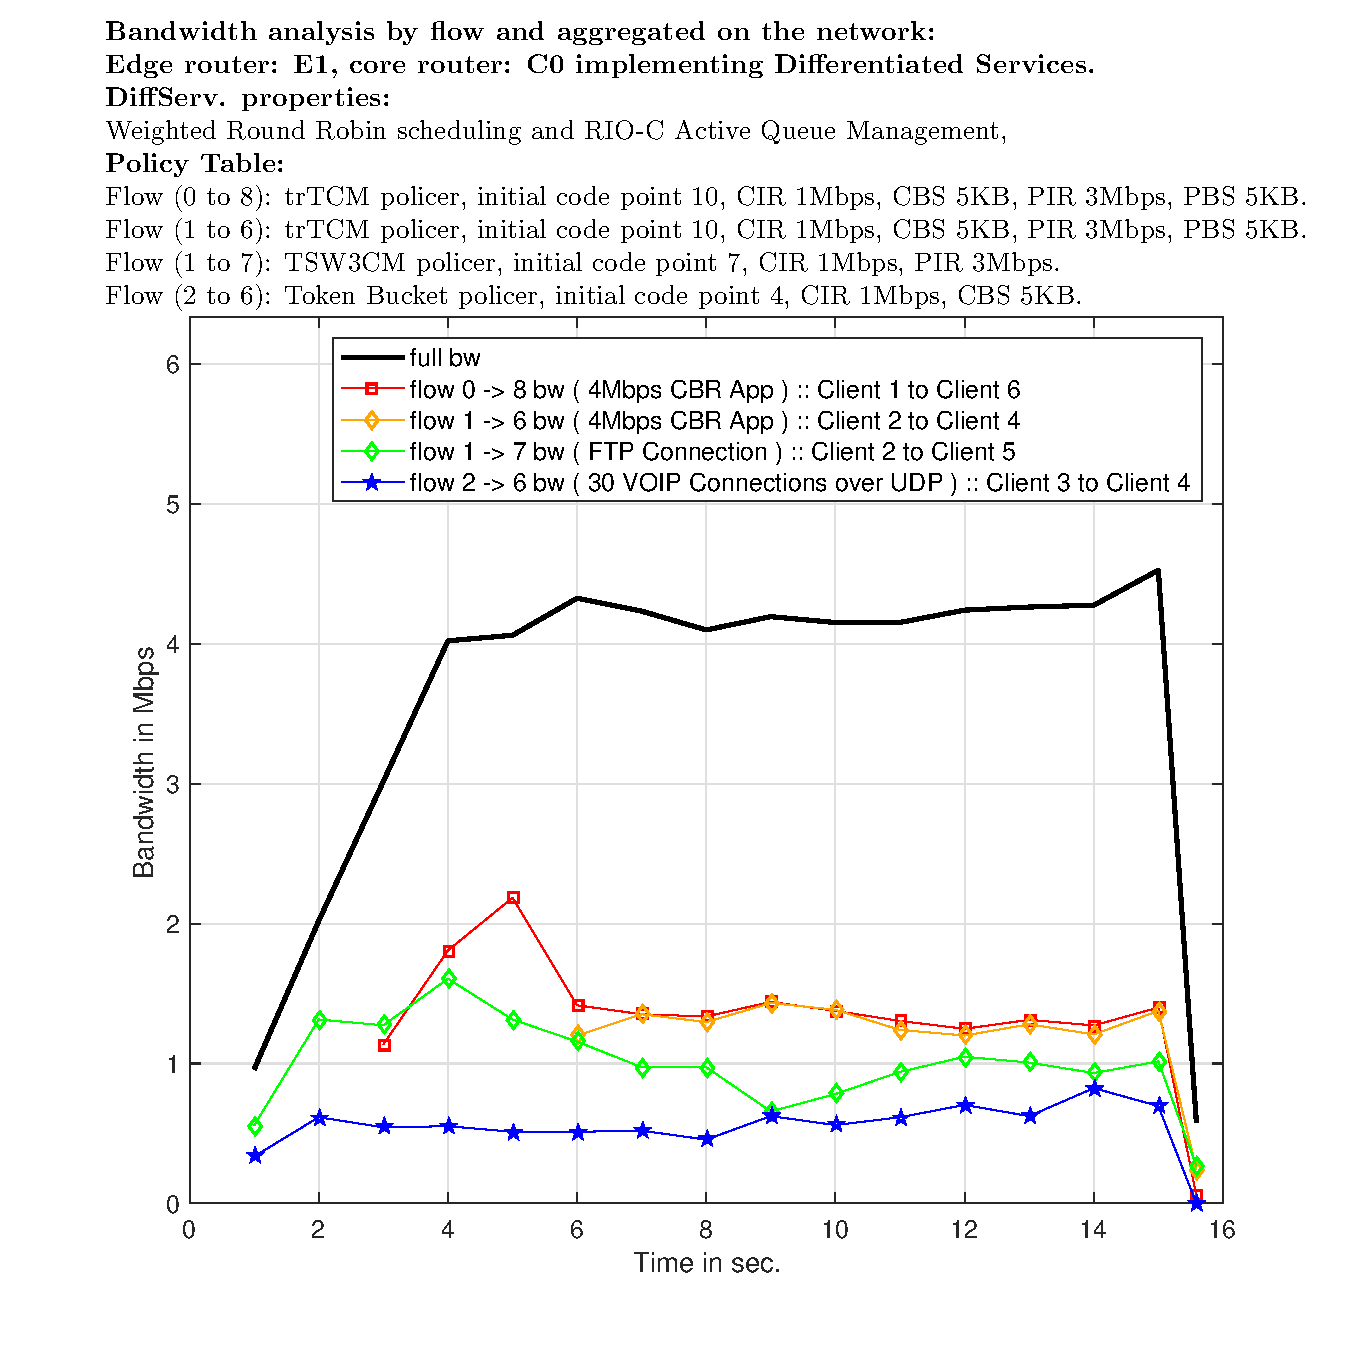
\includegraphics[width=1\columnwidth]{EPS/C/bw_c5_e1.eps}
     \caption{Bandwidth analysis by flow and aggregated, for edge router E1 and core router C0, implementing Differentiated Services.}
     \label{graph:bw_c5_e1}
     \end{figure}

\begin{figure}[H]
     \centering
     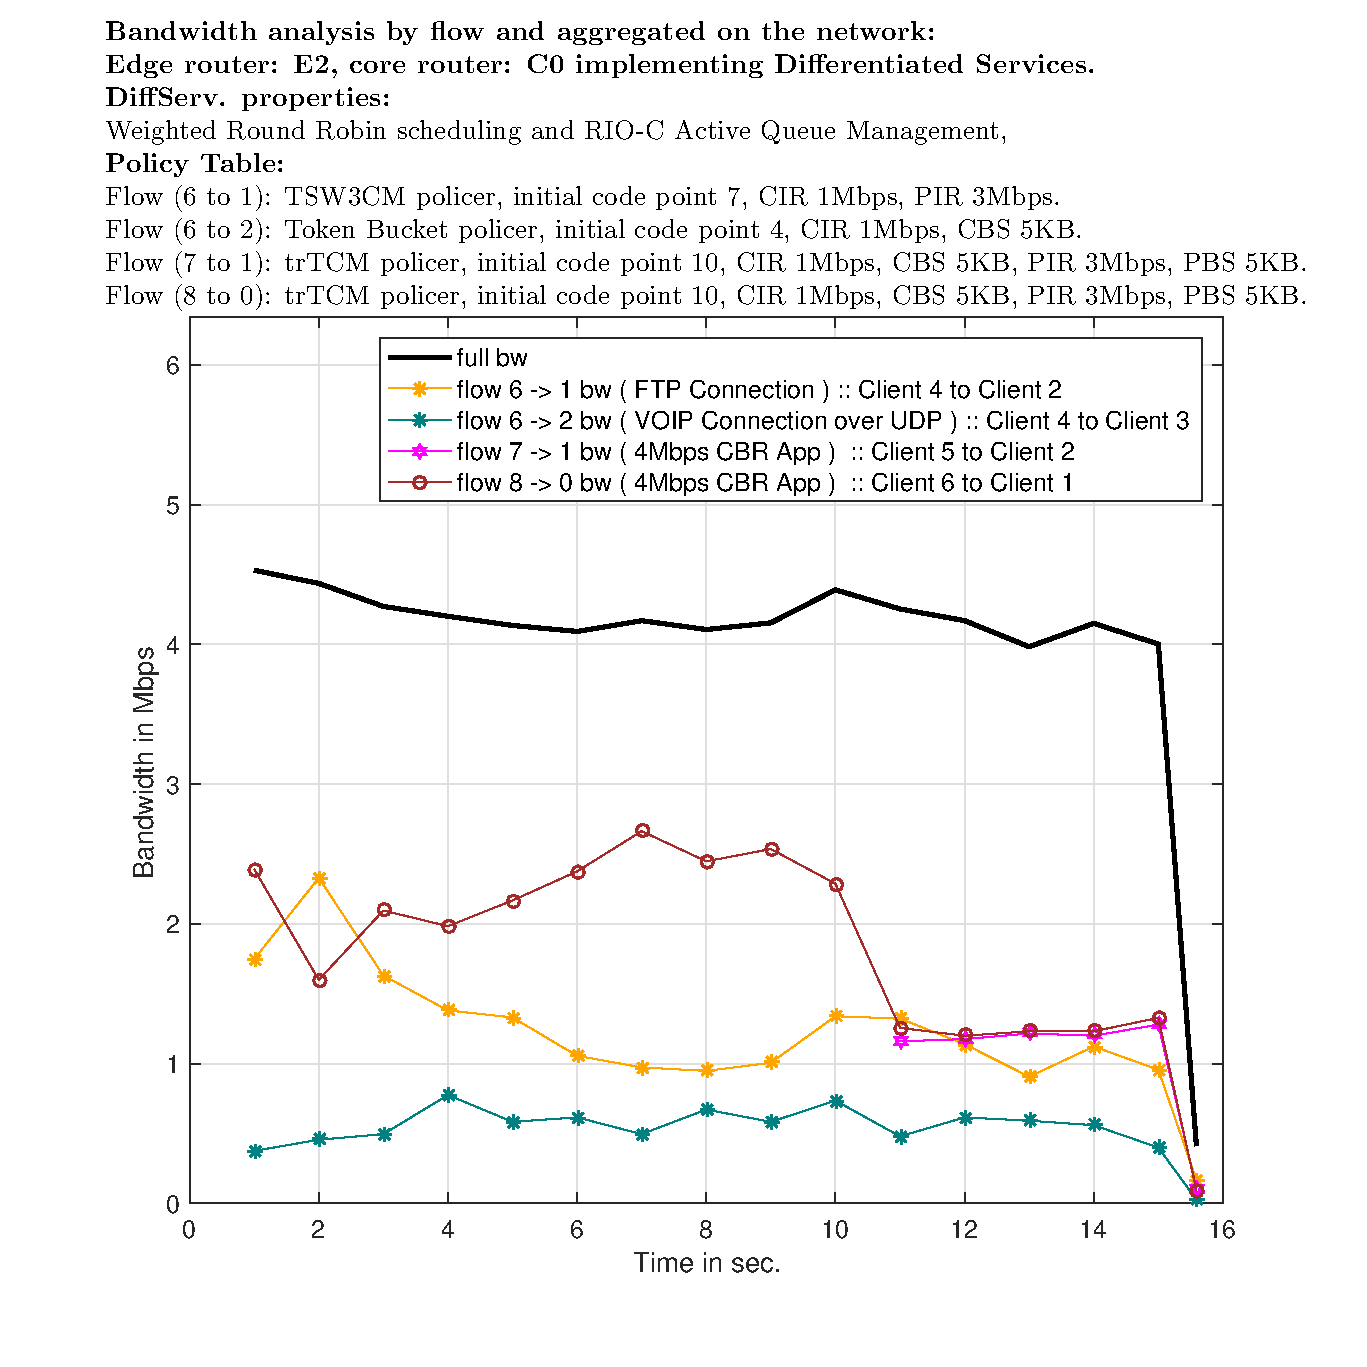
\includegraphics[width=1\columnwidth]{EPS/C/bw_c5_e2.eps}
     \caption{Bandwidth analysis by flow and aggregated, for edge router E2 and core router C0, implementing Differentiated Services.}
     \label{graph:bw_c5_e2}
     \end{figure}
     

     \begin{figure}[H]
     \centering
     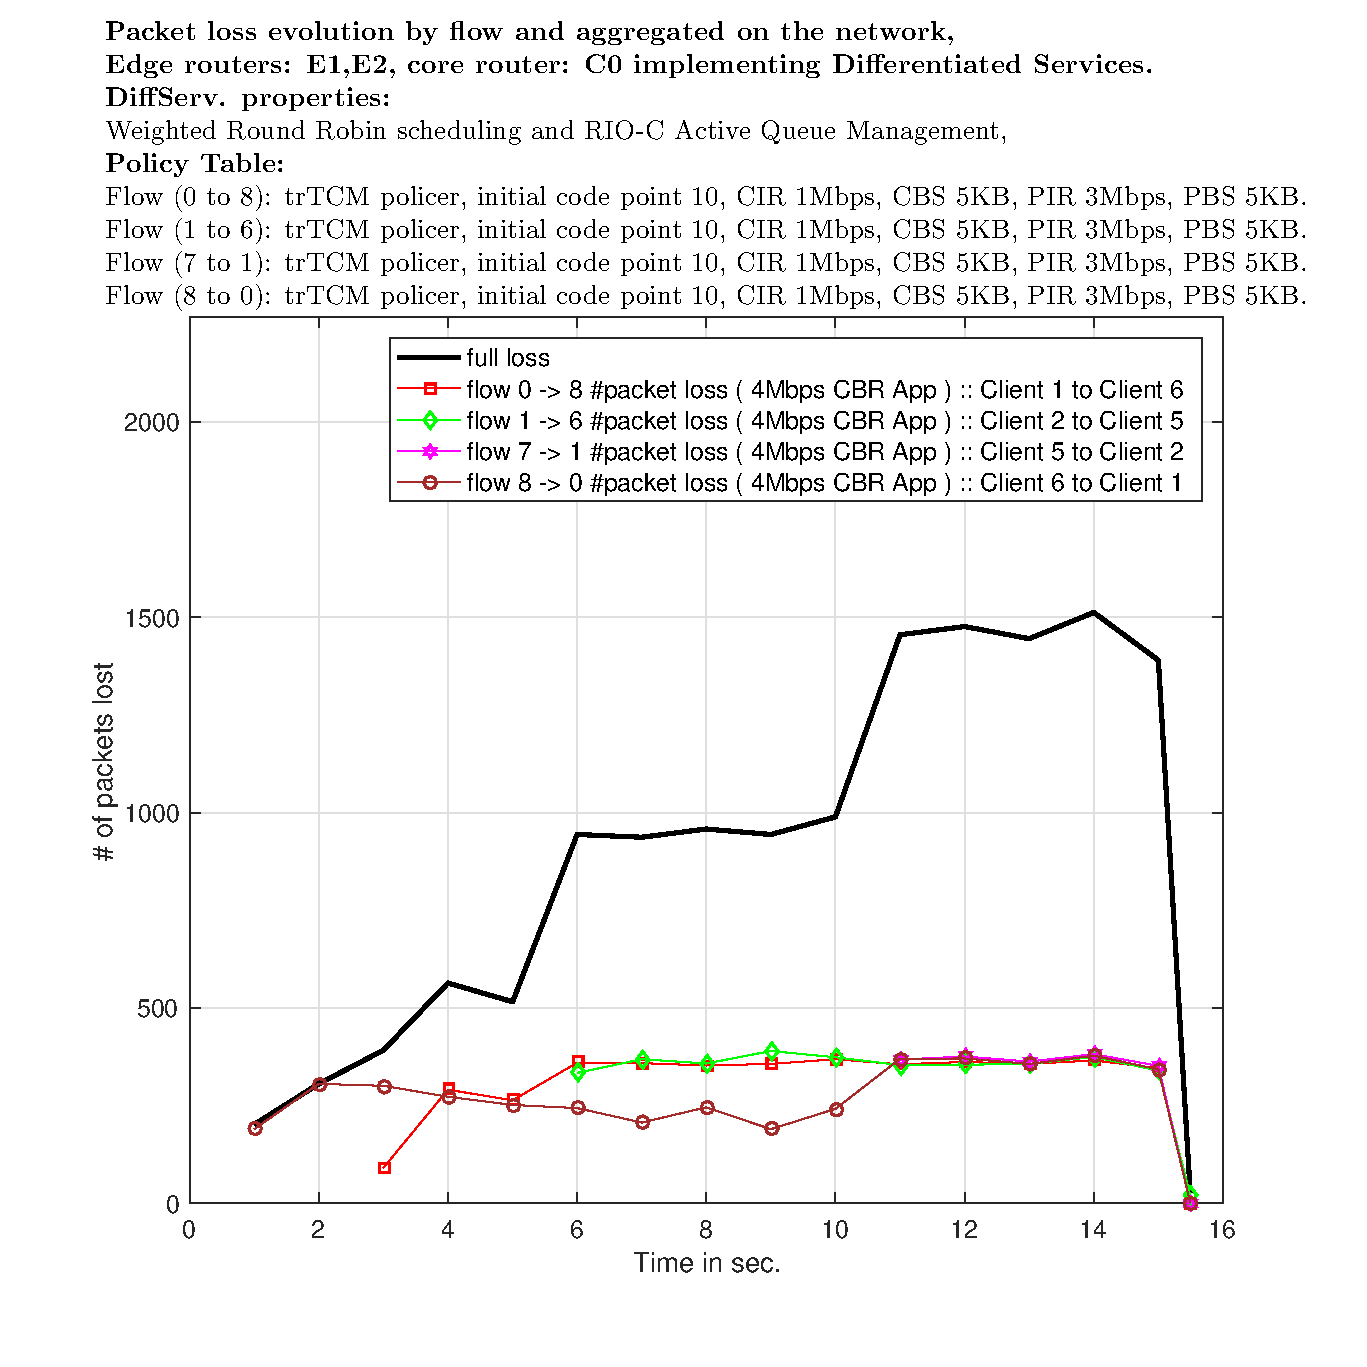
\includegraphics[width=1\columnwidth]{EPS/C/loss_c5.eps}
     \caption{Packet loss evolution by flow and aggregated, with edge/core routers implementing Differentiated Services.}
     \label{graph:loss_c5}
     \end{figure} 
     
     As you can stated by analysing figures \ref{graph:bw_c5_e1} and \ref{graph:bw_c5_e2}, despite the late start, all traffic from the same class has the same equitable bandwidth distribution -- as desired. We can also stated, by analysing figure \ref{graph:loss_c5},  that an increase in the total packets sent by flows only influences the packet drop of its traffic class. 
     
     
\subsubsection{Identification of the queue which suffers higher packet loss}.

\\Taking into account the simulation results/statistics, presented on tables \ref{table:c5_e1_c0_5s} to \ref{table:c5_c0_e2_15s}, we can identify the queue which suffers higher packet loss -- physical queue 2 and virtual queue 1 (CBR traffic downgrade (yellow)), from E1 to C0 (Edge $\rightarrow$ Core Configuration). The network behaviour is the expected one. As you can state all UDP and FTP traffic is delivered, and only the CBR traffic exceeding CIR is dropped  in congestion. \subsubsection{Statistics for time = 5s}
.
\begin{table}[H]
     \caption{Statistics for the queue from E1 to C0 (Edge $\rightarrow$ Core Configuration) }
     \label{table:c5_e1_c0_5s}
     \centering
     \begin{tabular}{ | L{1cm} | R{1.0cm} | R{1.0cm} | R {1.0  cm} | R {1.0  cm} |}
     \hline  CP & TotPkts &  TxPkts  & ldrops &  edrops \\ \hline \hline     
All  &   4250  &   3918   &   196   &   136\\ \hline
4     & 362   &   362   &     0   &     0\\ \hline
5    &    1     &   1     &   0      &  0\\ \hline
7    &  664   &   664    &    0    &    0\\ \hline
8     & 334   &   334      &  0      &  0\\ \hline
10  &   1644    & 1644 &       0    &    0\\ \hline
11   &  1245  &    913  &    196    &  136\\ \hline
\end{tabular}
\end{table}

\begin{table}[H]
     \caption{Statistics for the queue from C0 to E2 (Core $\rightarrow$  Edge Configuration) }
     \label{table:c5_c0_e2_5s}
     \centering
     \begin{tabular}{ | L{1cm} | R{1.0cm} | R{1.0cm} | R {1.0  cm} | R {1.0  cm} |}
     \hline  CP & TotPkts &  TxPkts  & ldrops &  edrops \\ \hline \hline
All&     3890   &  3890     &   0      &  0\\ \hline
4   &   362   &   362  &      0   &     0\\ \hline
5    &    1    &    1   &     0   &     0\\ \hline
7   &   664    &  664  &      0     &   0\\ \hline
8  &    333    &  333    &    0    &    0\\ \hline
10  &   1625   &  1625    &    0   &     0\\ \hline
11     & 905  &    905     &   0    &    0\\ \hline
     \end{tabular}
     \end{table}
     
 
 
 \subsubsection{Statistics for time = 10s}
.
\begin{table}[H]
     \caption{Statistics for the queue from E1 to C0 (Edge $\rightarrow$ Core Configuration) }
     \label{table:c5_e1_c0_10s}
     \centering
     \begin{tabular}{ | L{1cm} | R{1.0cm} | R{1.0cm} | R {1.0  cm} | R {1.0  cm} |}
     \hline  CP & TotPkts &  TxPkts  & ldrops &  edrops \\ \hline \hline
    All  &    8599  &    7957 &      312  &     330\\ \hline
4    &   726   &    726   &      0    &     0\\ \hline
5     &    1    &     1    &     0    &     0\\ \hline
7  &    1266  &    1266    &     0    &     0\\ \hline
8   &    792   &    792    &     0   &      0\\ \hline
10  &    3319  &    3319    &     0   &      0\\ \hline
11   &   2495  &    1853   &    312  &     330\\ \hline
     \end{tabular}
     \end{table}

\begin{table}[H]
     \caption{Statistics for the queue from C0 to E2 (Core $\rightarrow$  Edge Configuration) }
     \label{table:c5_c0_e2_10s}
     \centering
     \begin{tabular}{ | L{1cm} | R{1.0cm} | R{1.0cm} | R {1.0  cm} | R {1.0  cm} |}
     \hline  CP & TotPkts &  TxPkts  & ldrops &  edrops \\ \hline \hline
All  &    7938   &   7938    &     0    &     0\\ \hline
4   &    724    &   724    &     0    &     0\\ \hline
5   &      1      &   1  &       0     &    0\\ \hline
7 &     1266    &  1266    &     0    &     0\\ \hline
8   &    792  &     792  &       0    &     0\\ \hline
10  &    3308 &     3308   &      0   &      0\\ \hline
11   &   1847   &   1847  &       0   &      0\\ \hline
     \end{tabular}
     \end{table}
     
 

 \subsubsection{Statistics for time = 15s}
.

\begin{table}[H]
     \caption{Statistics for the queue from E1 to C0 (Edge $\rightarrow$ Core Configuration) }
     \label{table:c5_e1_c0_15s}
     \centering
     \begin{tabular}{ | L{1cm} | R{1.0cm} | R{1.0cm} | R {1.0  cm} | R {1.0  cm} |}
     \hline  CP & TotPkts &  TxPkts  & ldrops &  edrops \\ \hline \hline
     
  All   & 12911  &  12027    &  357   &   527\\ \hline
4  &   1021   &  1021 &       0    &    0\\ \hline
5    &    1    &    1    &    0    &    0\\ \hline
7  &   1864   &  1864     &   0    &    0\\ \hline
8   &  1264   &  1264  &      0   &     0\\ \hline
10  &   5016  &   5016     &   0   &     0\\ \hline
11 &    3745   &  2861   &   357   &   527\\ \hline
     \end{tabular}
     \end{table}
 
 
\begin{table}[H]
     \caption{Statistics for the queue from C0 to E2 (Core $\rightarrow$  Edge Configuration) }
     \label{table:c5_c0_e2_15s}
     \centering
     \begin{tabular}{ | L{1cm} | R{1.0cm} | R{1.0cm} | R {1.0  cm} | R {1.0  cm} |}
     \hline  CP & TotPkts &  TxPkts  & ldrops &  edrops \\ \hline \hline
  All &   12006  &  12006  &      0    &    0\\ \hline
4   &  1020  &   1020   &     0     &   0\\ \hline
5     &   1     &   1    &    0    &    0\\ \hline
7   &  1861  &   1861  &      0   &     0\\ \hline
8   &  1258    & 1258   &     0   &     0\\ \hline
10   &  5012  &   5012   &     0    &    0\\ \hline
11  &   2854  &   2854     &   0  &      0\\ \hline
     \end{tabular}
     \end{table}
     
     
\section{Conclusion}


In today’s multi-service networks, more and more complex applications are deployed
and QoS-sensitive data is growing in it. 
In this exploratory essay,  we reduced link congestion and end-to-end delays that multi-service networks  suffers from. \par 
Our proposed solution implied an full understanding of the network topology (something unfeasible in the real world). This ensured that high-priority traffic had the less loss percentage, and minimised the average percentage of packets lost during packet transmission. This resulted in improved network throughput and better QoS. \par 
However, as stated, this essay has low real-world scenario applications, being considered as an introductory mean to QoS terms and applications in multi-service networks to the authors.
     
\begin{thebibliography}{4}





\bibitem{ns} 
network simulator—ns (version 2). [Online]. Available:\\
\url{
https://sourceforge.net/projects/nsnam/files/allinone/ns-allinone-2.35/
}

\bibitem{manual} 
\\The ns Manual [Online]. Available:\\
\url{
http://www.isi.edu/nsnam/ns/doc/ns_doc.pdf
}

\bibitem{beginners} 
Altman E, and Jimenez T., (2003). NS Simulator for Beginners. Lecture notes. Univ.de Los Andes, Merida, Venezuela and ESSI.Sophia-Antipolis, France.\\

\bibitem{intro} 
T. Issariyakul, Introduction to Network Simulator NS2, Springer, 2008.




\end{thebibliography}
     \end{document}


